\documentclass[paper=a4,11pt,titlepage,twoside=true,headings=normal,numbers=noenddot,captions=tableabove,listof=totoc,index=totoc,bibliography=totoc, ngerman]{scrreprt}
%-----------------------------------------------------------------
\usepackage{etoolbox}
\newbool{deutsch}
\booltrue{deutsch}	% comment out to switch document to english
%-----------------------------------------------------------------
\usepackage{scrhack} % Improving Third-Party Packages with scrhack https://ctan.mc1.root.project-creative.net/macros/latex/contrib/koma-script/doc/scrguide-en.pdf
\usepackage{microtype} % Subliminal refinements towards typographical perfection https://ctan.org/pkg/microtype
\usepackage[reqno,intlimits]{amsmath} % [reqno] um die gleichungsnummerierung rechts zu haben
% intlimits: Grenzen für Integrale unterhalb und oberhalb des Zeichens
\usepackage{amssymb} % math symbols
\usepackage{array} % Extending the array and tabular environments https://ctan.org/pkg/array
\ifbool{deutsch}{%
    \usepackage[ngerman]{babel}
}{%
    \usepackage[english]{babel}
}
\usepackage{lmodern} % Latin modern fonts in outline formats https://www.ctan.org/pkg/lm
\usepackage[T1]{fontenc} % Standard package for selecting font encodings https://ctan.org/pkg/fontenc
\usepackage[utf8]{inputenc} % Accept different input encodings https://ctan.org/pkg/inputenc
\usepackage{csquotes}
\usepackage{libertine}
\usepackage{booktabs} % Publication quality tables in LaTeX https://ctan.org/pkg/booktabs
% \usepackage{calc} % Simple arithmetic in LaTeX commands https://ctan.org/pkg/calc
\usepackage[labelfont={footnotesize,sf,bf},textfont={footnotesize,sf}]{caption} % Customising captions in floating environments https://ctan.org/pkg/caption
%normalsize
%scriptsize
% sc --> smallcaps
% bf --> bold face
% sf --> sans serif
% \usepackage[table]{xcolor} % Driver-independent color extensions for LaTeX and pdfLaTeX https://ctan.org/pkg/xcolor
\usepackage{currency} % Format currencies in a consistent way https://ctan.org/pkg/currency
\DefineCurrency{EUR}{name={Euro},plural={Euro},iso={EUR},kind=iso,symbol={\€}}
\usepackage{ellipsis} % Fix uneven spacing around ellipses in LaTeX text mode https://ctan.org/pkg/ellipsis
\usepackage{graphicx} % Enhanced support for graphics https://ctan.org/pkg/graphicx
% \usepackage{listings} % Typeset source code listings using LaTeX https://ctan.org/pkg/listings
\usepackage{lastpage} % Reference last page for Page N of M type footers https://ctan.org/pkg/lastpage
% \usepackage{makeidx} % Standard LaTeX package for creating indexes https://www.ctan.org/pkg/makeidx
% \usepackage{paralist} % Enumerate and itemize within paragraphs https://www.ctan.org/pkg/paralist
\usepackage[automark]{scrlayer-scrpage} % Define and manage page styles https://www.ctan.org/pkg/scrlayer-scrpage
\usepackage[locale=DE,per-mode=power,range-units=repeat,separate-uncertainty=true]{siunitx} % A comprehensive (SI) units package https://www.ctan.org/pkg/siunitx
\DeclareSIUnit\amperehour{Ah}
\DeclareSIUnit\watthour{Wh}
\DeclareSIUnit\newtonmetre{Nm}
\usepackage{subcaption} % Support for sub-captions https://www.ctan.org/pkg/subcaption
\usepackage{threeparttable} % better tablenotes
\usepackage{tabularx} % Tabulars with adjustable-width columns https://www.ctan.org/pkg/tabularx
\usepackage{tocbasic} % Management of tables/lists of contents (and the like) https://www.ctan.org/pkg/tocbasic
\usepackage{url}
\usepackage{xurl} % Allow URL breaks at any alphanumerical character https://www.ctan.org/pkg/xurl
\usepackage{wrapfig} % Produces figures which text can flow around https://www.ctan.org/pkg/wrapfig
% \usepackage{varioref} % Intelligent page references https://ctan.org/pkg/varioref
\usepackage{hyperref} % Extensive support for hypertext in LaTeX https://www.ctan.org/pkg/hyperref
\hypersetup{
    pdftitle={Konzeption und Realisierung eines Antriebssystems für ein elektrisches Longboard},
    pdfauthor={Dennis Hunter},
    pdfsubject={Projektarbeit},
    bookmarksopen=true,
    bookmarksnumbered=true,
    colorlinks=true, % Color links instead of disgusting boxes :barfing_emoji:
    linkcolor={black}, % Color of internal links
    citecolor={black}, % Color of citations
    urlcolor={blue} % Color of external hyperlinks
}
\usepackage{cleveref} % Intelligent cross-referencing https://www.ctan.org/pkg/cleveref
\crefname{equation}{Gl.}{Gl.}
\Crefname{equation}{Gleichung}{Gleichungen}
\usepackage[style=IEEE, citestyle=numeric, backend=biber, date=short]{biblatex} % Sophisticated Bibliographies in LaTeX https://www.ctan.org/pkg/biblatex
\urlstyle{same}
\setcounter{biburllcpenalty}{100}
\setcounter{biburlucpenalty}{200}
\setcounter{biburlnumpenalty}{100}
\usepackage[useregional]{datetime2} % Formats for dates, times and time zones https://www.ctan.org/pkg/datetime2
\usepackage[inkscapearea=page]{svg} % Include and extract SVG pictures in LaTeX documents https://ctan.org/pkg/svg
\usepackage[numbered]{bookmark} % A new bookmark (outline) organization for hyperref https://www.ctan.org/pkg/bookmark
% ---------- Make floats stay within the chapter/section/subsection they got placed ------------------
\usepackage{placeins} % Control float placement https://www.ctan.org/pkg/placeins
\let\Oldsection\section
\renewcommand{\section}[1]{\FloatBarrier\Oldsection{#1}}
\let\Oldsubsection\subsection
\renewcommand{\subsection}[1]{\FloatBarrier\Oldsubsection{#1}}
\let\Oldsubsubsection\subsubsection
\renewcommand{\subsubsection}[1]{\FloatBarrier\Oldsubsubsection{#1}}
%===================== define VARIABLES ==========================
% --------------------- Names ------------------------------------
\newcommand{\thefirstnameA}{Dennis}
\newcommand{\thelastnameA}{Hunter}
\newcommand{\thefirstnameB}{Dung}
\newcommand{\thelastnameB}{Pie}
\newcommand{\thefirstnameC}{Donkey}
\newcommand{\thelastnameC}{Shorts}
% --------------------- Titel Course -----------------------------
\newcommand{\titleLV}{Projektarbeit}
%---------------------- Document Titel ---------------------------
\newcommand{\subtitleA}{Konzeption und Realisierung eines Antriebssystems für ein elektrisches Longboard}
\newcommand{\subtitleB}{``MotherBoard''}
%-------------- Deprecated below but still usable ----------------
%---------------------- Dates ------------------------------------
% \newcommand{\versuch}{2} % Versuchsnummer einfügen
% \newcommand{\dateLV}{17.11.2020} % Datum einfügen
% \newcommand{\deadline}{28.02.2022} % Abgabedatum ist der 1.12.2020
% \newcommand{\dateLVa}{December 1st, 2020}
% \newcommand{\dateLVb}{December 8th, 2020}
%:::::::::::::::::::::::::::::::::::::::::::::::::::::::::::::::::
%A4: 210x297 (BxH)
% \setlength{\voffset}{-2.532 cm}
% \setlength{\hoffset}{-1.57 cm}
\setlength{\voffset}{-2.5 cm}
\setlength{\hoffset}{-2 cm}
% \setlength{\topmargin}{2.0 cm} \setlength{\topskip}{0.1 cm}
\setlength{\topmargin}{1.5 cm}
\setlength{\topskip}{0.1 cm}
\setlength{\evensidemargin}{1.5 cm}
\setlength{\oddsidemargin}{1.5 cm}
%  \setlength{\textwidth}{16.5 cm}
\setlength{\textwidth}{16.0 cm}
\setlength{\footskip}{40pt}
\setlength{\textheight}{24.7cm}
% \setlength{\textheight}{23.5 cm}
\setcounter{page}{1}
\setlength{\parindent}{0.5cm}
\setlength{\headsep}{20pt}
%------------------ Kopf- und Fusszeilen
\setkomafont{pageheadfoot}{\footnotesize\sffamily}
% \renewcommand{\footnote}[1]{\footnote{\quad#1}}
\counterwithout{footnote}{chapter}
%------------------------------------------------------------------------
% Linien in der Kopf- und Fußzeile
%\renewcommand{\headrulewidth}{0.0pt}   %Linie in der Kopfzeile mit 0.0pt keine Linie
%%\renewcommand{\footrulewidth}{0.0pt}   %Linie in der Fußzeile mit 0.0 pt keine Linie
%\renewcommand{\headrulewidth}{0.2pt}   %Linie in der Kopfzeile mit 0.0pt keine Linie
%\renewcommand{\footrulewidth}{0.2pt}   %Linie in der Fußzeile mit 0.0 pt keine Linie
%------------------------------------------------------------------------
%\renewcommand{\normalfont}{\sffamily} %für die Überschriften
%\renewcommand{\chaptermark}[1]{\markboth{\chaptername\ \thechapter #1}{}}
%\renewcommand{\sectionmark}[1]{\markright{\thesection\ #1}}
% \rfoot{\leftmark\\\rightmark}

%Definitionen für Kopfzeile
% bei documentclass {report} hat der Eintrag für die [gerade Seite] keine Wirkung
%-------------------------------------------------------------
%%
%Einstellungen für Kopf- und Fusszeilen mit dem KOMA-Skript und \usepackage{scrpage2}
\pagestyle{scrheadings}
%\pagestyle{scrplain}
% le --> links, gerade Seite
% ce --> mittig, gerade Seite
% re --> rechts, gerade Seite
% lo --> links, ungerade Seite
% co --> mittig, ungerade Seite
% ro --> rechts, ungerade Seite
%---------------------------------------------
% Löschen aller Einträge
%\clearscrheadings
% \automark[section]{subsection}
% \pagemark --> Seitenzahl
% \automark --> Kapitelüberschriften
% \leftmark --> ??
% \rightmark --> ??
%::::::::::::::::::::::::::::::::::: Kopfzeile
% Kopfzeile gerade Seite
\automark[chapter]{chapter}
\lehead[]{\titelkopfzeilelinkseven}
\cehead[]{\titelkopfzeilemitteeven}
\rehead[]{\titelkopfzeilerechtseven}
% Kopfzeile ungerade Seite
\lohead[]{\titelkopfzeilelinksodd}
\cohead[]{\titelkopfzeilemitteodd}
\rohead[]{\titelkopfzeilerechtsodd}
% Linie in der Kopfzeile
%\setheadtopline{0.2pt} % obere Linie in der Kopfzeile; nur bei scrartcl
%\setheadsepline{0.4pt} % untere Linie in der Kopfzeile; nur bei scrartcl
\KOMAoptions{headsepline=0.4pt}
% Linie in der Fusszeile
%::::::::::::::::::::::::::::::::::: Fußzeile
% Fusszeile gerade Seite[plain-style]{scrheadings-style}
\lefoot[]{\titelfusszeilelinkseven} 
\cefoot[]{\titelfusszeilemitteeven}
\refoot[]{\titelfusszeilerechtseven}
% Fusszeile ungerade Seite
\lofoot[]{\titelfusszeilelinksodd}
\cofoot[]{\titelfusszeilemitteodd}
\rofoot[]{\titelfusszeilerechtsodd}
%\rofoot[\thepage ]{\thepage}
%\setfoottopline{0.2pt} % obere Linie in der Kopfzeile; nur bei scrartcl
%\setfootsepline{0.4pt} % untere Linie in der Kopfzeile; nur bei scrartcl
\KOMAoptions{footsepline=0.4pt}

% le --> links, gerade Seite
% ce --> mittig, gerade Seite
% re --> rechts, gerade Seite
% lo --> links, ungerade Seite
% co --> mittig, ungerade Seite
% ro --> rechts, ungerade Seite
% even --> gerade Seite
% odd --> ungerade Seite
%----------------------------------------- Kopfzeilentext
 \newcommand{\titelkopfzeilemitteeven}{}
 \newcommand{\titelkopfzeilemitteodd}{}
 \newcommand{\titelkopfzeilelinkseven}{Hochschule RheinMain}
 \newcommand{\titelkopfzeilelinksodd}{}
 \newcommand{\titelkopfzeilerechtseven}{}
 \newcommand{\titelkopfzeilerechtsodd}{Hochschule RheinMain}
 %----------------------------------------- Fußzeilentext
 \newcommand{\titelfusszeilemitteeven}{}
 \newcommand{\titelfusszeilemitteodd}{}
 \newcommand{\titelfusszeilerechtseven}{Studienbereich Angewandte Physik \& Medizintechnik}
 \newcommand{\titelfusszeilerechtsodd}{\thepage \hspace{0.5mm} von~\pageref{LastPage}}
 \newcommand{\titelfusszeilelinkseven}{\thepage \hspace{0.5mm} von~\pageref{LastPage}}
 \newcommand{\titelfusszeilelinksodd}{Studienbereich Angewandte Physik \& Medizintechnik}
\ifbool{deutsch}{%
    \usepackage[intoc,german]{nomencl}\makenomenclature % Produce lists of symbols as in nomenclature https://www.ctan.org/pkg/nomencl
    \renewcommand{\nomgroup}[1]{%
    \ifstrequal{#1}{A}{\item[\textbf{Abkürzungen}]}{%
    \ifstrequal{#1}{G}{\vspace{20pt}\item[\textbf{Griechische Zeichen}]}{%
    \ifstrequal{#1}{L}{\vspace{20pt}\item[\textbf{Lateinische Zeichen}]}{}}}%
    }%
    \renewcommand{\nomname}{Nomenklatur}
}{%
    \usepackage[intoc]{nomencl}\makenomenclature
    \renewcommand{\nomgroup}[1]{%
    \ifstrequal{#1}{A}{\item[\textbf{Abbreviations}]}{%
    \ifstrequal{#1}{G}{\vspace{20pt}\item[\textbf{Greek Symbols}]}{%
    \ifstrequal{#1}{L}{\vspace{20pt}\item[\textbf{Roman Symbols}]}{}}}%
    }%
    \renewcommand{\nomname}{Nomenclature}
}
\newcommand{\nomunit}[1]{%
\renewcommand{\nomentryend}{\hspace*{\fill}\(\left[\unit{#1}\right]\)}}
\setlength{\nomitemsep}{.3\parsep}
% %
%=====================Code Listing Layout Matlab=============================
\definecolor{codegreen}{RGB}{28,172,0} % color values Red, Green, Blue
\definecolor{codelilas}{RGB}{170,55,241}
\lstdefinestyle{matlab}{language=Matlab,%
    basicstyle=\footnotesize,%
    inputencoding=latin1,%
    breaklines=true,%
    stepnumber=2,% line numbering steps
    morekeywords={ones,height,width,datetime},% additional keywords to highlight
    keywordstyle=\color{blue},%
    frame=none,%
    identifierstyle=\color{black},%
    stringstyle=\color{codelilas},%
    commentstyle=\color{codegreen},%
    showstringspaces=false,%without this there will be a symbol in the places where there is a space
    numbers=left,%
    numberstyle={\tiny \color{black}},% size of the numbers
    numbersep=9pt,% this defines how far the numbers are from the text
}
\lstdefinestyle{python}{language=Python,%
    basicstyle=\footnotesize,%
    inputencoding=latin1,%
    breaklines=true,%
    stepnumber=2,% line numbering steps
    morekeywords={ones,height,width,datetime},% additional keywords to highlight
    keywordstyle=\color{blue},%
    frame=none,%
    identifierstyle=\color{black},%
    stringstyle=\color{codelilas},%
    commentstyle=\color{codegreen},%
    showstringspaces=false,%without this there will be a symbol in the places where there is a space
    numbers=left,%
    numberstyle={\tiny \color{black}},% size of the numbers
    numbersep=9pt,% this defines how far the numbers are from the text
}
%==============================================================================
\DeclareNameAlias{author}{family-given}
\DeclareNameAlias{editor}{family-given}
\DeclareNameAlias{translator}{family-given}
\addbibresource{literature.bib}
%------DEBUGGING--------------------------------------------------
% \usepackage[showframe]{geometry} % comment out for live version
% \usepackage{layout}
% \usepackage{showframe}
% \usepackage[export]{adjustbox} % adds aside others the <frame> option to \includegraphics[]{}. this makes there borders visible and helps debugging/aligning
%-----------------------------------------------------------------
\begin{document}
%-----------------------------------------------------------------
% Original author:
% Peter Wilson (herries.press@earthlink.net) with modifications by:
% Vel (vel@latextemplates.com)
%
% License:
% CC BY-NC-SA 3.0 (http://creativecommons.org/licenses/by-nc-sa/3.0/)
%
% Original found under:
% https://www.latextemplates.com/template/formal-book-title-page
\hypersetup{pageanchor=false}
\begin{titlepage}
	%------------------------------------------------
	%	Names
	%------------------------------------------------
	\ifbool{deutsch}{%
		\newcommand{\nameA}{\thefirstnameA\space\thelastnameA}
		\newcommand{\nameB}{\thefirstnameB\space\thelastnameB}
		\newcommand{\nameC}{\thefirstnameC\space\thelastnameC}
	}{%
		\newcommand{\nameA}{\thelastnameA,\space\thefirstnameA}
		\newcommand{\nameB}{\thelastnameB,\space\thefirstnameB}
		\newcommand{\nameC}{\thelastnameC,\space\thefirstnameC}
	}

	%------------------------------------------------
	%	General format
	%------------------------------------------------
	\centering
	\vspace*{\baselineskip} % White space at the top of the page
	{
		\scshape % Use small caps for all text on the title page

		%------------------------------------------------
		%	Title
		%------------------------------------------------
		\vspace*{\baselineskip} % White space at the top of the page
		\rule{\textwidth}{1.6pt}\vspace*{-\baselineskip}\vspace*{2pt} % Thick horizontal rule
		\rule{\textwidth}{0.4pt} % Thin horizontal rule
		\vspace{0.75\baselineskip} % Whitespace above the title

		{\huge \textbf{\subtitleA}}\par\vspace{0.4cm} % Title of Document
		{\huge \textbf{\subtitleB}}\par\vspace{0.4cm} % Titel des Dokuments

		\vspace{0.75\baselineskip} % Whitespace below the title
		\rule{\textwidth}{0.4pt}\vspace*{-\baselineskip}\vspace{3.2pt} % Thin horizontal rule
		\rule{\textwidth}{1.6pt} % Thick horizontal rule
		\vspace{2\baselineskip} % Whitespace after the title block

		%------------------------------------------------
		%	Subtitle
		%------------------------------------------------
		\textsc{\Large \titleLV}\vspace{0.5cm}%
		\vspace*{3\baselineskip} % Whitespace under the subtitle

		%------------------------------------------------
		%	Authors
		%------------------------------------------------
		\ifbool{deutsch}{%
			\underline{Autor}\par\vspace{0.5cm}
		}{%
			\underline{Author}\par\vspace{0.5cm}
		}
		\vspace{0.5\baselineskip} % Whitespace above the editors
		{\scshape\LARGE \nameA} % Editor list
		\vspace{0.5\baselineskip} % Whitespace below the editor list

		%------------------------------------------------
		%	Publisher
		%------------------------------------------------
		\ifbool{deutsch}{%
			Hochschule RheinMain \\ Fachbereich Ingenieurwissenschaften \\ Studienbereich Angewandte Physik \& Medizintechnik
		}{%
			Hochschule RheinMain \\ Department of Engineering \\ Applied Physics \& Medical Technology
		}
		\vfill % Whitespace between editor names and publisher logo

		\begin{center}
			
\includegraphics[width=0.15\textwidth]{logo-hsrm.jpg} % Logo
		\end{center}
		\vspace{0.3\baselineskip} % Whitespace under the logo
		\today % Publication year
	}
\end{titlepage}
\shipout\null%
\hypersetup{pageanchor=true}
\clearpage\pagenumbering{Roman}
\tableofcontents
\listoffigures
\listoftables
\printnomenclature[5cm]
%-----------------------------------------------------------------
\clearpage\pagenumbering{arabic}
% LTeX: language=de-DE
\chapter{Einleitung}
% ===============================================
% Nomenclatures
% ===============================================
\nomenclature[A]{PEKV}{Persönliche elektrische Kleinstvehikel}%
\nomenclature[A]{ePKW}{Elektrische Personenkraftwagen}%
\nomenclature[A]{PEV}{Persönliche elektrische Vehikel}%
%
	Weltweit findet derzeit auf politischer wie gesellschaftlicher Ebene ein Umdenken im Transportwesen statt --~sei es der Transport von Gütern, Fahrgästen oder im Individualverkehr.
	Angefeuert durch den unmittelbaren monetären Druck durch steigende Treibstoffpreise, die immer deutlicher werdenden Folgen fortdauernder CO\textsubscript{2}-Emissionen aber auch Lebensqualität beeinflussende Faktoren wie Staus und abnehmende Luftqualität in urbanen Gebieten treibt eine wachsende Zahl Menschen aus Auto heraus auf alternative Transportmöglichkeiten.
	Neben der klassischen Möglichkeit des Fahrrades kam mit erheblichen Verbesserungen und der deutlich breiteren Verfügbarkeit der Lithiumbatterie-Technologie ein Wandel des gesellschaftlichen Lebens einher, wie es vergleichbar zuletzt geschah, als das Smartphone die Bühne der Welt betrat -~die Elektrifizierung des Individualverkehrs.
	Nachdem einige Vorreiterstädte bereits früh mit baulichen Maßnahmen etwa durch Herabsetzen innerörtlicher Geschwindigkeitsbegrenzungen, Ausbau von Fahrradwegen oder Zuwachs öffentlicher Verkehrsmittel reagierten, ziehen nun immer mehr Städte nach.
	Dieser wechselseitige Trend bildet sich auch in der politischen Stimmung ab mit einer der wichtigsten Novellen für das öffentliche Verkehrsbild, die die ``\textit{Verordnung über die Teilnahme von Elektrokleinstfahrzeugen am Straßenverkehr und zur Änderung weiterer straßenverkehrsrechtlicher Vorschriften}'' von 2019 mit sich zog~\cite{Bundesgesetzblatt.2019}.
	Sie leutete den Advent breit verfügbarer persönlicher elektrischer Kleinstvehikel (PEKV) zur Überbrückung der ``letzten Meile'' ein.\par\medskip
	%
	Die Kategorie elektrifizierter persönlicher Fahrzeuge lässt sich grob unterteilen in elektrische Personenkraftwagen (ePKW), persönliche elektrische Vehikel (PEV) und --~wie oben bereits erwähnt~-- die persönlichen elektrischen Kleinstvehikel in der kleinsten Variante.
	Zwar dominiert die erste Gruppe gegenwärtige politische Bemühungen zum Thema, gerade im städtischen Raum bieten sie jedoch kaum bis kein Potenzial, Infarkte des Straßenverkehrs zu vermeiden.
	Die Ladeinfrastruktur ist noch nicht einheitlich und flächendeckend geregelt und allem voran sind sie preislich für breite Teile der Bevölkerung unattraktiv.
	Vielversprechender sind Vertreter der beiden letztgenannten Gruppen.
	Dem Statistischen Bundesamt zufolge besaßen zu Jahresanfang~2020 etwa jeder neunte deutsche Haushalt oder \SI{11,4}{\percent} zumindest ein elektrisch angetriebenes Fahrrad.
	Während sie Anfang 2015 mit \(\sim \SI{4}{\percent}\) noch in etwa jedem 25. Haushalt aufzufinden waren, kann hier eine Verbreitung um fast das Dreifache verzeichnet werden~\cite{zahl.der.ebikes.StatistischesBundesamt.2020.09.28}.\par\medskip
% LTeX: language=de-DE
\chapter{Konzeption}\label{sec:conception}
	%
	Um Konsistenz mit Literatur und Marktrecherchen sicherzustellen werden im Rahmen dieser Arbeit technische Begriffe aus der Skaterszene genutzt.
	Während Skateboarding einerseits keinesfalls als neuartiges Phänomen zu bezeichnen ist und andererseits in den vergangenen fünf Jahren eine Renaissance erlebt hat, kann, gerade im nicht-englischsprachigen Raum, nicht davon ausgegangen werden, dass alle Lesenden mit der Terminologie vertraut sind.
	Daher wird im Folgenden zunächst Fokus auf eine Begriffskonvention gelegt und in diesem Rahmen funktionale Kernkomponenten eines Skate- bzw. Longboards\footnote{\hspace{1mm} Baulich zwar leicht zu unterscheiden, jedoch aus den gleichen Kernkomponenten und -funktionalitäten aufgebaut.}~erläutert.\par\medskip
	%
	Das Antriebssystem soll in ein vorgegebenes, übergeordnetes System bestehend aus mechanischen und elektronischen Komponenten eingebettet werden.
	Sowohl das übergeordnete System, als auch die Einsatzumgebung definieren konstruktive Einschränkungen, die in einem weiteren Unterkapitel herausgearbeitet werden sollen.\par\medskip
	%
	Zuletzt werden vor dem Hintergrund zuvor festgelegter Rahmenbedingungen und unterstützt durch Markt- und Literaturrecherche Designziele definiert und erste Designideen konkretisiert.
	%
	\section{Funktionale Komponenten eines Longboards}
		%
		Historisch ergaben sich esoterische lautende Namenskonventionen für Teilkomponenten von Skate- und Longboards.
		Während sie im einfachsten Fall unabhängig des Sprachraumes mit ihren jeweiligen englischen Begriffen zu finden sind, weichen Bezeichnungen bisweilen stark von in der Industrie verbreiteten Bezeichnungen ab.
		Um jener Namenskonvention zu folgen, sollen hier zunächst die Teilkomponenten kurz beschrieben werden.\par\medskip
		%
		\begin{figure}[h]
			\centering
			\includesvg[width=.9\textwidth]{Footage/AwesomeBoard Transmission CAD/Drawings/Longboard.svg}
			\caption[Grundlegender Aufbau eines Longboards]{Grundlegender Aufbau eines Longboards. 15~Deck, 16~Truck Bolts, 17~Truck Bolt Nuts, 18~Riser Pad.}\label{fig:longboard}
		\end{figure}
		%
		\Cref{fig:longboard} zeigt den grundlegenden Aufbau eines Longboards.
		Erkennbar sind hier vordergründig das Deck~(15), welches die fahrende Person trägt und hierbei einen Großteil der wirkenden Kräfte aufnehmen muss.
		Je nach Fahrstil werden weichere oder härtere Materialien gewünscht um etwa Unebenheiten des Untergrundes auszugleichen oder die Ausführung von Tricks\footnote{\hspace{1mm} Über die rein laterale Fortbewegung hinausgehende, meist kunstvoll ausgeführte Bewegungen des Boards mit und unter den Füßen.}~positiv zu beeinflussen.

		Meist kommt hier Schichtholz mit oder ohne eingearbeiteten Glas-, Aramid- oder Kohlefasergewebes zum Einsatz, es sind bisweilen aber auch exotischere Materialien wie Aluminium oder ABS\footnote{\hspace{1mm} Acrylnitrilbutadienstyrol.}~vertreten.\nomenclature[A]{ABS}{Acrylnitrilbutadienstyrol}
		In \cref{fig:longboard} befinden sich links und rechts, zentral entlang der Längsachse des Decks angeordnet die Trucks genannten Baugruppen zusammen mit jeweils zwei Rollen.
		Eine mechanisch belastbare Verbindung zum Deck wird durch Truck Bolts~(16) und Truck Bolt Nuts~(17) hergestellt.
		Gegenüber den mit deutlich kleineren Rollen ausgestatteten Skateboards ist es im Longboarding üblich zwischen Deck und Truck Riser Pads~(18) einzusetzen.
		Hierbei handelt es sich um aus flexiblem Material verschiedener Härtegrade gefertigte Pufferplatten mit Doppelfunktion:
		Einerseits unterstützen sie die Entkopplung der Füße von Vibration und verhindern andererseits sogenannte Wheel Bites -~ein Kontakt des Decks mit den Rollen während eines Lenkmanövers mit meist fataler Konsequenz.

		%
		\begin{figure}[h]
			\centering
			\includesvg[width=.9\textwidth]{Footage/AwesomeBoard Transmission CAD/Drawings/Drivetrain - Truck}
			\caption[Explosionsansicht eines der Trucks]{Aufbau eines der Trucks als Explosionsansicht exemplarisch an einem \textsc{Caliper II}. Sichtbar sind hier: 1~Baseplate, 2~Pivot Cup, 3~Kingpin, 4~Hanger, 5~RS Bushing, 6~BS Bushing, 7~BS Washer, 8~RS Washer, 9~Kingpin Nut.}\label{fig:caliper exploded}
		\end{figure}
		%
		Der Aufbau der Trucks selbst wird in \cref{fig:caliper exploded} exemplarisch am Typ \textsc{Caliber II} gezeigt.
		Der Hanger~(4) bildet hier das zentrale Bauteil und muss den Großteil der wirkenden Kräfte aufnehmen.
		Er wird drehbar und gleitend in der Baseplate~(1) gelagert.
		Direkter Kontakt zwischen Hanger und Baseplate hätte erhöhten Abrieb und reduziertes Gleitverhalten zur Konsequenz wozu hier ein meist aus POM\footnote{\hspace{1mm} Polyoxymethylen.}~gefertigter Pivot Cup~(2) eingesetzt wird.
		In Position gehalten wird der Hanger mittels Kingpin~(3) und Kingpin Nut~(9).
		Das Rückstellmoment nach Ende eines Lenkmanövers wird durch zwei Bushings --~vergleichsweise dicke Gummiringe -- erzeugt, die mit der Kingpin-Achse koaxial beidseitig mit dem Hanger in mechanischem Kontakt stehen.
		Deckseitig befindet sich der BS Bushing~(6), straßenseitig angeordnet der RS Bushing.\nomenclature[A]{BS}{Board Side}\nomenclature[A]{RS}{Road Side}
		Die Präfixe stehen für Board Side bzw. Road Side und spiegeln ihre Positionen wider.
		Unterschieden wird hier, da sich verschiedene Geometrien und Härtegrade der Bushings abhängig ihrer Position merklich auf das Fahrgefühl und Lenkvermögen auswirken können\footnote{\hspace{1mm} Durch Drehen der Kingpin Nut und damit einer Änderung der Vorspannung der Bushings~kann hier auch im Feld relativ unkompliziert nachjustiert werden}.
		Um die Lasten flächig auf die Oberfläche der Bushings zu verteilen, werden RS und BS Washer~(7,8), üblicherweise tellerförmige Scheiben, auf der dem Hanger abgewandten Seite platziert.\par\medskip
		%
		\begin{figure}[h]
			\centering
			\includesvg[width=.9\textwidth]{Footage/AwesomeBoard Transmission CAD/Drawings/Drivetrain - Wheels NT}
			\caption[Montage der Rollen an der Achse des Hanger]{Montage der Rollen an der Achse des Hangers. Links in explodierter und rechts in Schnittansicht. Zu sehen sind: 10~Rolle, 11~Kugellager, 12~Speedring, 13~Spacer, 14~Achsmutter.}\label{fig:wheel NT exploded}
		\end{figure}
		%
		Je nach gewünschter Laufruhe und in Abwägung zwischen Traktion und Rollwiderstand werden Rollen verschiedener Größen und Materialien drehbar auf den Hanger-Achsen gelagert.
		Mit Blick auf \cref{fig:wheel NT exploded} wird konzentrisch in den Kern der Rolle~(10) --~vergleichbar mit einer Felge, die das weichere Mantelmaterial trägt --~beidseitig jeweils ein Radialrillenkugellager~(11) platziert.
		Hier hat sich historisch über quasi-sämtliche Rollenbauerten hinweg das 608-Kugellager durchgesetzt.
		Um potenziell den Lagern gegenüber destruktive axiale Kräfte in Kurven oder durch das Anzugsmoment der Achsmutter~(14) zu minimieren, wird, ebenfalls in den Kern der Rolle und zwischen die beiden Lager, der Spacer~(13) angeordnet.
		Er besteht aus hartem Metall, hat einen Innendurchmesser gleich des nominellen Durchmessers der Hanger-Achse, eine Wandstärke von \(\sim \qty{1}{\milli\metre}\) und eine Länge, die gerade so gewählt ist, dass er an beiden Flanken mit den Innenringen der Lager in Kontakt steht, wenn sie beide vollständig im Kern eingelassen sind.
		Ein schleiffreies Laufen der Lager wird durch Speedrings~(12) sichergestellt.
		Ihre Dimensionen entsprechen denen des Spacers, allerdings mit einer deutlich geringeren Länge von nur \qty{1}{\milli\metre}.
		Letztlich werden alle Komponenten mit einer Achsmutter auf der Hanger-Achse fixiert.
		%
	\section{Konstruktive Rahmenbedingungen}\label{sec:constructive limitations}
		%
		Das Antriebssystem soll in ein bestehendes System aus Batterie, Batteriemanagement, Motorcontrollern und Deck integriert und an die Einsatzbedingungen angepasst werden.
		Hieraus ergeben sich bei der Planung zu berücksichtigende konstruktive Rahmenbedingungen.
		%
		\subsection{Bestehendes System}
			%
			Die Batterie besteht aus 40~Lithium-Ionen Zellen in 10S4P-Konfiguration vom Typ \textsc{Samsung INR18650-30Q} mit einer nominellen Zellspannung von \qty{3,6}{\volt}, einer Mindestzellentladekapazität von \qty{2950}{\milli\amperehour} und einem maximalen Entladestrom von \qty{15}{\ampere} (vgl.~\cref{tab:cellspecifications}~\cite{INR18650.30Q.Specs.202202}).
			%
			\begin{table}[h]
				\caption[Zellspezifikationen \textsc{Samsung INR18650-30Q}]{Zellspezifikationen \textsc{Samsung INR18650-30Q}~\cite{INR18650.30Q.Specs.202202}.}%
				\label{tab:cellspecifications}
				\centering
				\begin{tabular}{p{.4\textwidth}l}
					\toprule
					Charakteristik				& Spezifikationen \\ \midrule
					Minimale Entladekapazität	& \qty{2950}{\milli\amperehour} \\
					Nominelle Zellspannung		& \qty{3,6}{\volt} \\
					Standard Ladebedingungen	& CC/CV, \qty{1,5}{\ampere}, \qty{4,2 +- 0,05}{\volt} \\
					Maximale Ladebedingungen	& CC/CV, \qty{4}{\ampere}, \qty{4,2 +- 0,05}{\volt} \\
					Maximaler Dauerentladestrom & \qty{15}{\ampere} bei \qty{25}{\degreeCelsius} \\
					Minimale Zellspannung		& \qty{2,5}{\volt} \\
					Gewicht						& \qty{48}{\gram} \\
					Betriebstemperatur			& Laden: \qtyrange{0}{50}{\degreeCelsius}, Entladen: \qtyrange{-20}{75}{\degreeCelsius} \\ \bottomrule
				\end{tabular}
			\end{table}
			%
			%
			10S4P meint hier jeweils vier Zellen parallel geschaltet mit 10 jener Sub-Zellen elektrisch in Serie (vgl.~hierzu~\cref{fig:battery pack}).
			So ergibt sich eine nominelle Spannung der Batterie von \qty{36}{\volt}, eine Kapazität von \qty{11,8}{\amperehour} und eine abrufbare Energie von \(\sim \SI{425}{\watthour}\) bei einem maximalen Dauerentladestrom von \SI{60}{\ampere}.
			\begin{figure}[h]
				\centering
				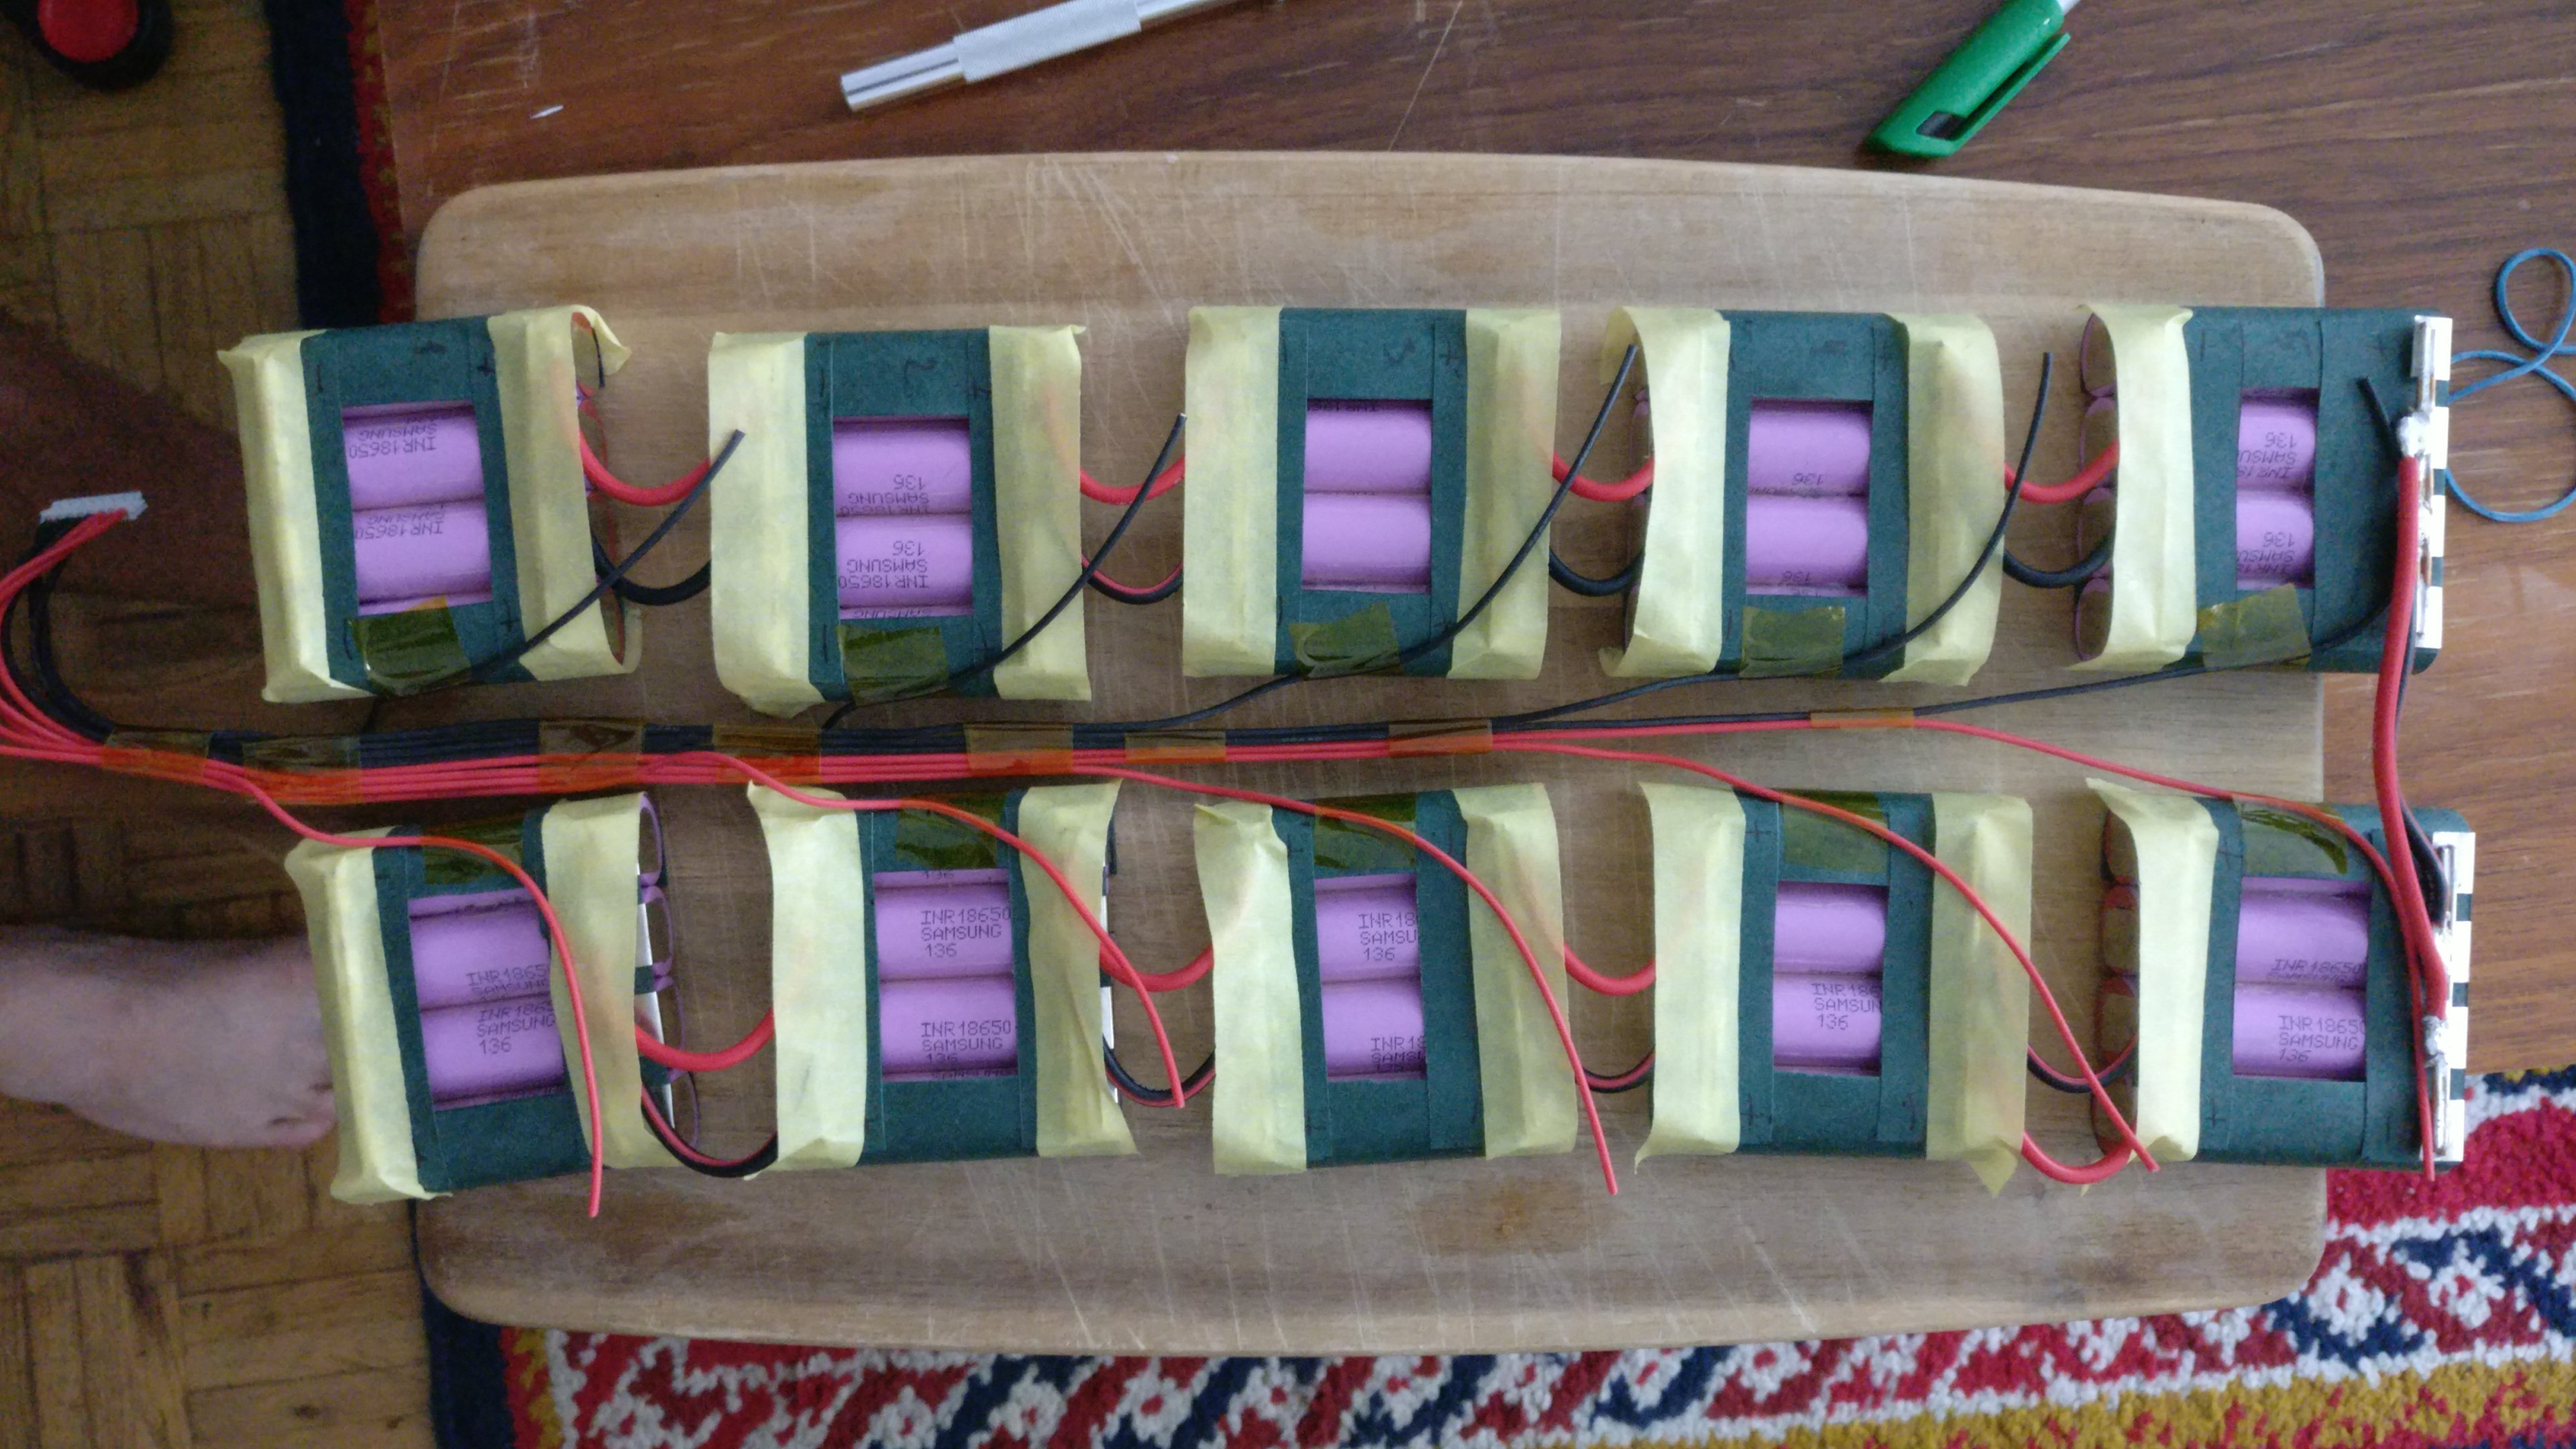
\includegraphics[width=.9\textwidth]{Footage/Pictures/Battery pack.jpg}
				\caption[Der verbaute Lithium-Ionen Zellverband]{Der verbaute Lithium-Ionen Zellverband. Zu erkennen sind die 10 Sub-Zellen bestehend aus jeweils vier Einzelzellen.}\label{fig:battery pack}
			\end{figure}

			%
			Das Drehmoment soll durch Elektromotoren erzeugt werden, die von zwei elektronischen Speed Controllern (ESC)\nomenclature[A]{ESC}{Elektronischer Speed Controller} des Typs \textsc{FSESC 4.12}\footnote{\hspace{1mm} Die wiederum industriell gefertigte 1:1 Nachbauten des populären Open-Source \textsc{VESC} von Benjamin~Vedder sind.} angesteuert werden.
			ESC sind elektronische Komponenten vornehmlich zur elektronischen Kommutation von bürstenlosen Gleichstrommotoren (Brushless Direct Current, BLDC).\nomenclature[A]{BLDC}{Brushless Direct Current}
			\begin{figure}[h]
				\centering
				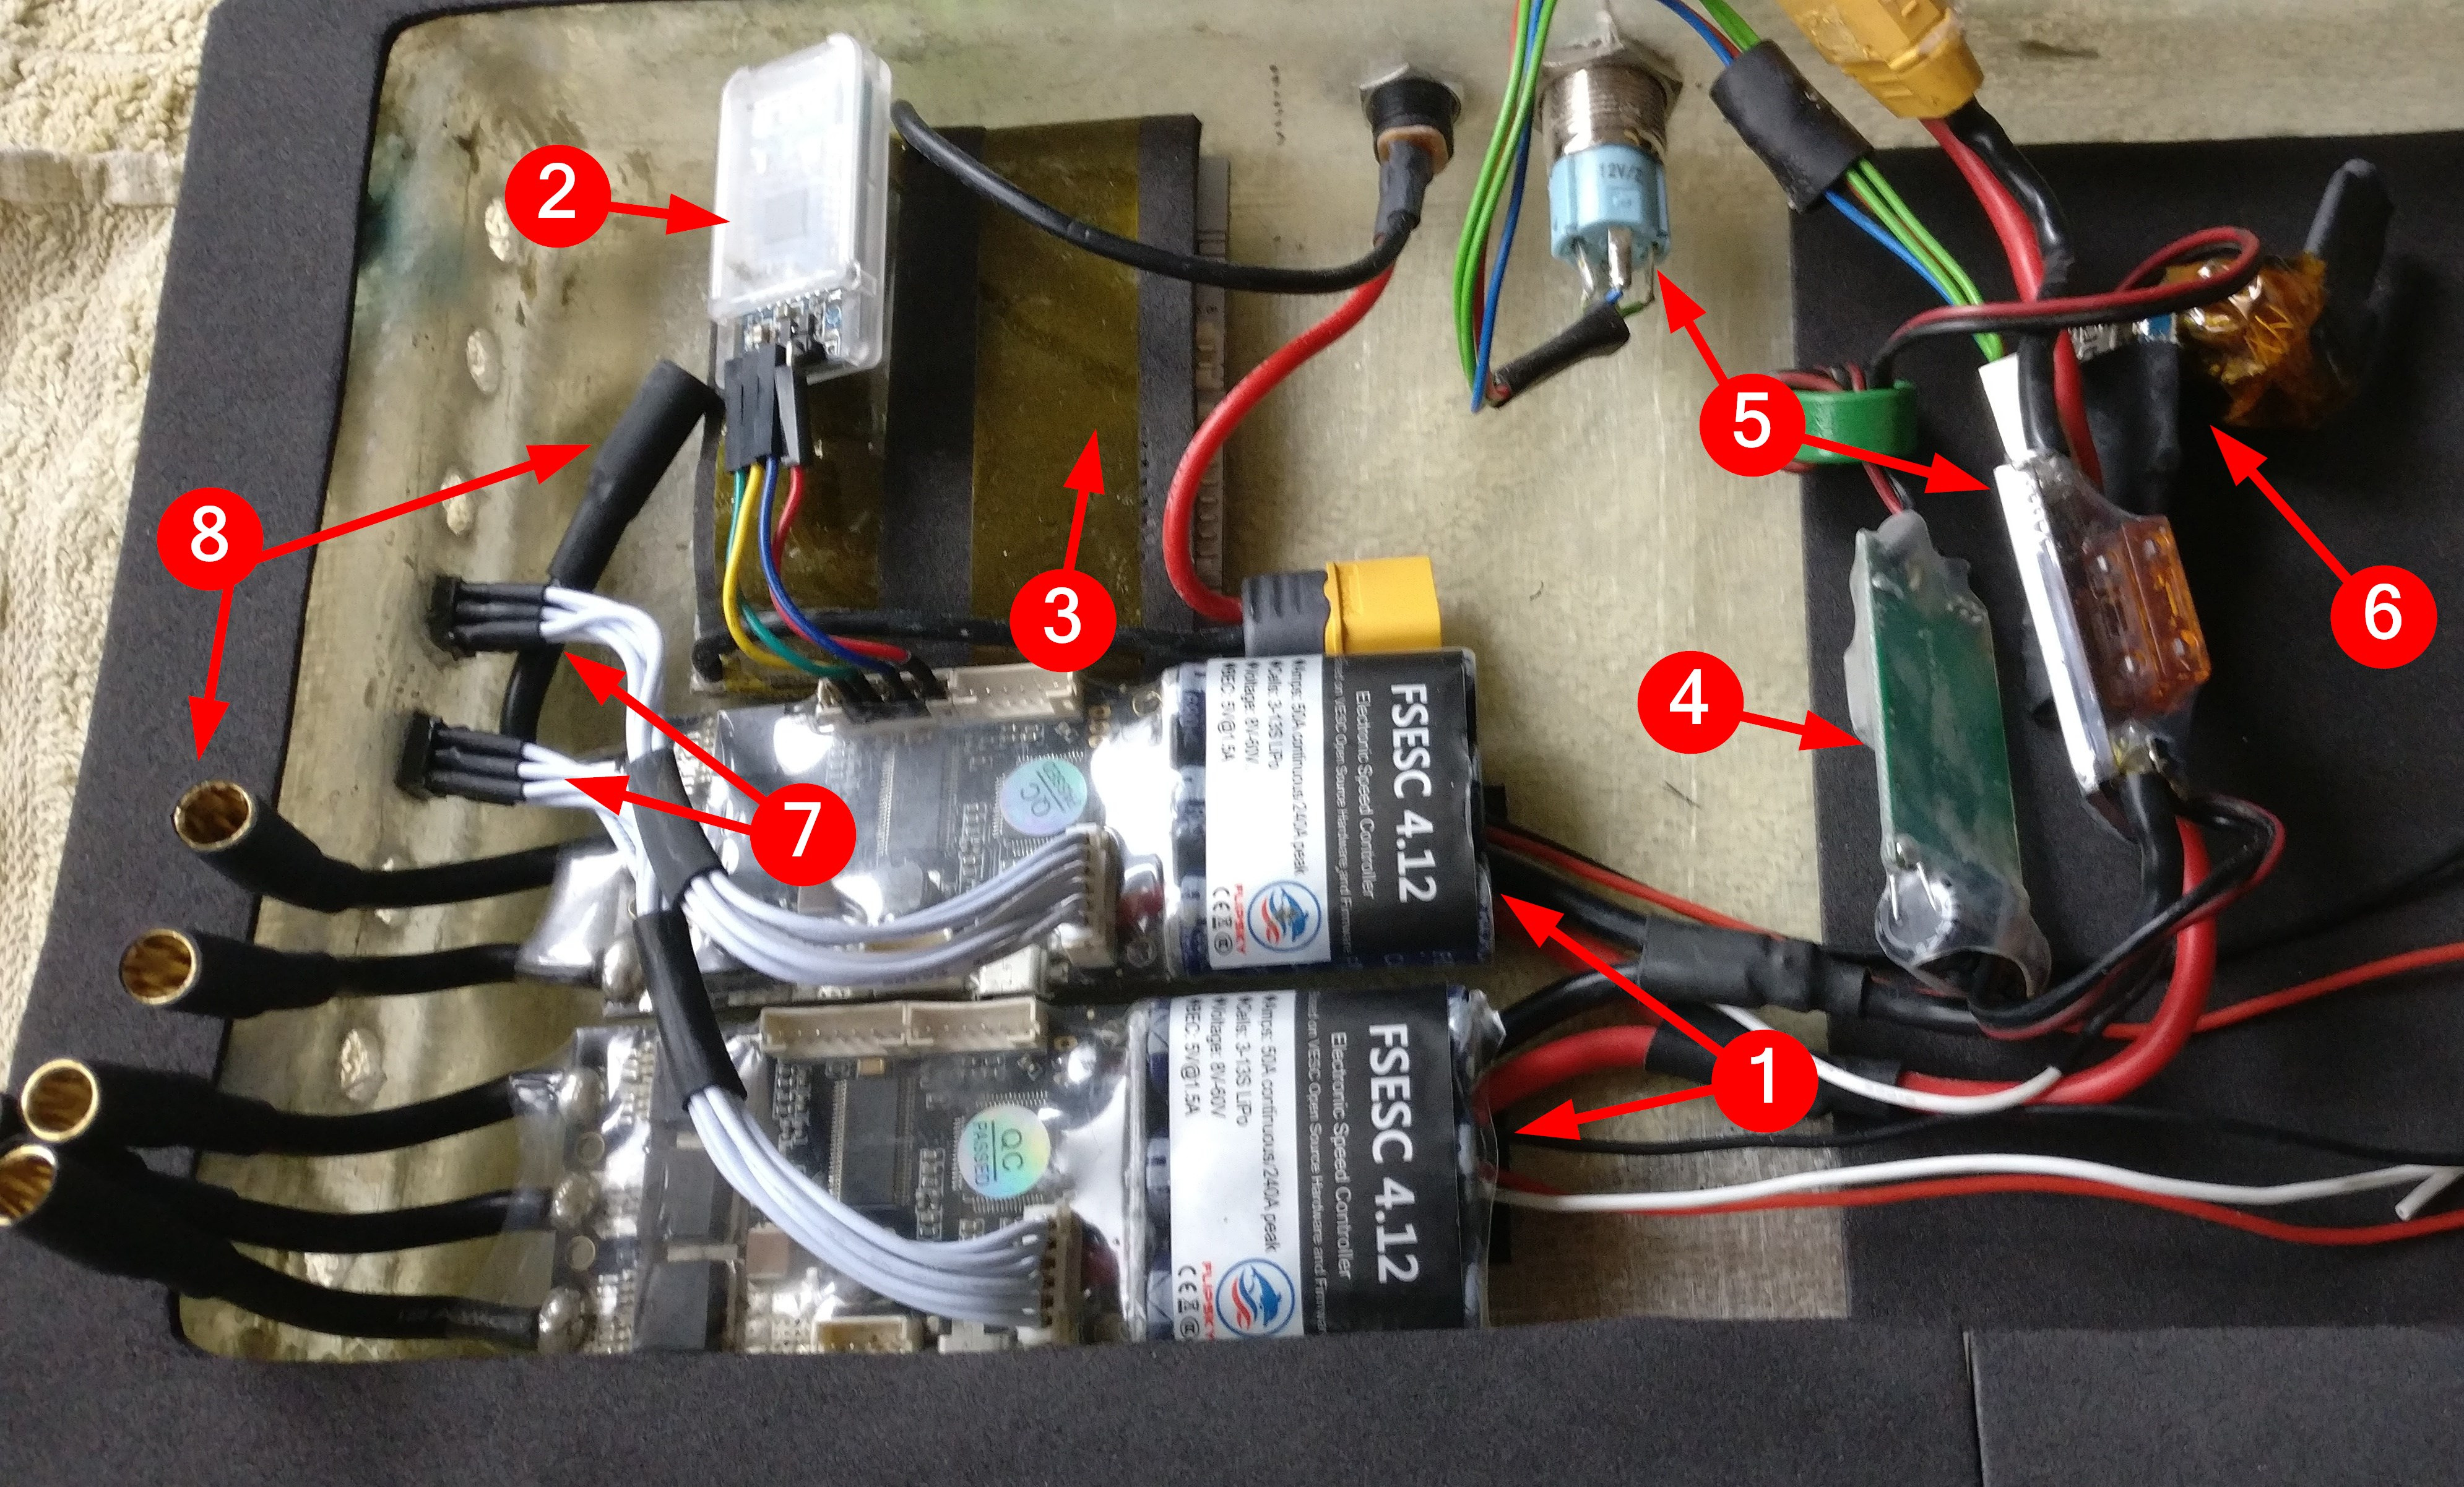
\includegraphics[width=.9\textwidth]{Footage/Pictures/Electronics.jpg}
				\caption[Eingesetzte ESC]{Unten im Bild die beiden eingesetzten ESC vom Typ \textsc{FSESC 4.12}. Weiterhin im Bild zu sehen oben links ein HC-06 Bluetooth Modul, darunter das Batteriemanagementsystem. Auf der rechten Seite im Bild von links nach rechts: Spannungsregler, elektronischer Schalter und der Funkempfänger für die Steuersignale.}\label{fig:electronics}
			\end{figure}
			Als solche schränken sie die Auswahl der Motortypen zwar nicht exklusiv auf BLDCs ein --~Gleichstrommotoren mit Schleifkontakt sind auch denkbar -- allerdings bieten sie in Kombination mit BLDCs einen deutlich höheren Funktionsumfang.
			Darüber hinaus sind BLDC gegenüber Gleichstrommotoren mit Schleifkontakten effizienter, bieten eine höhere Leistungsdichte, sind bauartbedingt unempfindlich gegenüber Nässe und quasi-wartungsfrei\footnote{\hspace{1mm} Je nach Art der Lagerung. Dies betrifft jedoch ausschließlich die mechanischen Komponenten der Motoren.}.
			%
		\subsection{Einsatzumgebung und -bedingungen}
			%
			Das Gewicht des Fahrers wird inklusive Kleidung und transportiertem Gepäck mit \qty{90}{\kilo\gram} angenommen.
			Hinzuzuaddieren sind \(\sim \qty{5}{\kilo\gram}\) durch Deck, Batterie und Elektronik und pessimistisch geschätzte weitere \qty{5}{\kilo\gram} durch die beiden Trucks zusammen mit dem Antriebssystem.
			So ergibt sich ein geschätztes, vom Antriebssystem zu beschleunigendes Gesamtgewicht von \(\sim \qty{100}{\kilo\gram}\)

			Weiter soll die fertige Maschine auf in urbanen Gebieten üblichen Untergründen betrieben werden können.
			Es wird also mit leichten bis moderaten Steigungen und in Form des Bodenbelages mit Asphalt und Kopfsteinpflaster gerechnet.\par\medskip
			%
			Die Maschine soll vorrangig als Sportgerät für milde bis sonnige Wetterlagen geeignet sein.
			Extrembedingungen wie Starkregen, Schnee oder Eisglätte finden hier keine weitere Beachtung.

	\section{Designziele}
		Mit in \cref{sec:constructive limitations} genannten Einschränkungen können einige Soll-Forderungen formuliert werden.
		So muss das System\ldots
		\begin{itemize}
			\item \ldots in der Lage sein, mindestens das angenommene Gesamtgewicht von \qty{100}{\kilo\gram} moderate Steigungen hinauf befördern zu können.
			Als Designrichtlinie wird hier eine Steigung von \qty{5}{\percent} festgelegt.
			\item \ldots entlang ebenen Asphaltes auf mindestens \qty{25}{\kilo\metre\per\hour} beschleunigen können.
			In Kombination mit obiger Forderung wird hier auf das Festlegen eines Zeitintervalls, innerhalb dessen die Endgeschwindigkeit erreicht werden soll, verzichtet.
			\item \ldots einfach zu Warten sein.
		\end{itemize}
		Neben den harten Zielen ist wünschenswert, dass das System\ldots
		\begin{itemize}
			\item \ldots möglichst aus selbst herstellbaren Komponenten besteht.
			\item \ldots kostengünstig ist.
			Als Richtwert soll hier \dEUR{300} angelegt werden.
			\item \ldots die von der Batterie zur Verfügung gestellte Energie von \SI{425}{\watthour} bezogen auf die erreichbare Reichweite möglichst effizient nutzt.
		\end{itemize}
% LTeX: language=de-DE
\chapter{Theorie}
	Die mechanische Gesamtleistung, die vom System auf den Boden übertragen werden muss ist die Summe unterschiedlicher Einzelfaktoren.
	Neben der erforderlichen Leistung, um die träge Masse von Maschine und Pilot aus dem Stand auf eine gewünschte Geschwindigkeit zu beschleunigen müssen zusätzliche Reserven zur Verfügung stehen, um mechanische Verluste wie Rollwiderstand zum Untergrund, bei höheren Geschwindigkeiten zunehmend aerodynamische Effekte oder Hangabtriebskräfte während des Befahrens von Steigungen überwinden zu können.\par
	Der Rollwiderstand wird beschrieben durch:
	\begin{align}
		F_{Roll} = m \cdot g \cdot c_{Roll}
		\label{eq:rolling resistance}
	\end{align}
	\nomenclature[L]{\(F_{Roll}\)}{Rollwiderstand\nomunit{\newton}}%
	\nomenclature[L]{\(m\)}{Masse\nomunit{\kilo\gram}}%
	\nomenclature[L]{\(g\)}{Erdbeschleunigung\nomunit{\metre\per\square\second}}%
	\nomenclature[L]{\(c_{Roll}\)}{Rollwiderstandkoeffizient\nomunit{1}}%
	mit dem dimensionslosen Rollwiderstandskoeffizienten \(c_{Roll}\) der wiederum das Verhältnis aus Rollreibungskoeffizienten \(\mu_{Roll}\)\nomenclature[G]{\(\mu_{Roll}\)}{Rollreibungskoeffizient\nomunit{\metre}} und dem Radius der Rollen nach \(\frac{\mu_{Roll}}{r}\) beschreibt.\par\medskip
	%
	Die Hangabtriebskraft mit dem Neigungswinkel \(\theta\)\nomenclature[G]{\(\theta\)}{Hangneigungswinkel\nomunit{rad}} ist gegeben durch:
	\begin{align}
		F_{Hang} = m \cdot g \cdot sin\left(\theta\right)
		\label{eq:downhill force}
	\end{align}
	\nomenclature[L]{\(F_{Hang}\)}{Hangabtriebskraft\nomunit{\newton}}%
	Die durch Reibung in Luft verursachte Kraft errechnet sich aus:
	\begin{align}
		F_{Ström} = \frac{1}{2} \cdot c_{Ström} \cdot \rho \cdot A \cdot v^2
		\label{eq:air drag}
	\end{align}
	\nomenclature[L]{\(F_{Ström}\)}{Strömungswiderstand\nomunit{\newton}}%
	\nomenclature[G]{\(\rho\)}{Gasdichte\nomunit{\kilo\gram\per\cubic\metre}}%
	\nomenclature[L]{\(A\)}{Fläche\nomunit{\square\metre}}%
	\nomenclature[L]{\(c_{Luft}\)}{Strömungswiderstandkoeffizient\nomunit{1}}%
	\nomenclature[L]{\(v\)}{Laterale Geschwindigkeit\nomunit{\metre\per\second}}%

	Darüber hinaus sind elektrische Verluste etwa im Serienwiderstand der Batterie, bei der Kommutation und bei der Ummagnetisierung der Phasenwicklungen zu berücksichtigen.
	Da diese im Einzelnen jedoch nur schwer quantifiziert werden können, sollen sie sich im Wirkungsgrad \(\eta\), der das Verhältnis aus abgerufener elektrischer Leistung zu umgesetzter mechanischer Leistung bildet, widerspiegeln.\par\medskip
	%
	Die Drehmomentkonstante \(K_T\)\nomenclature[L]{\(K_T\)}{Drehmomentkonstante\nomunit{\newton\metre\per\ampere}} eines BLDC berechnet sich aus der reziproken Drehzahlkonstante \(K_V\)\nomenclature[L]{\(K_V\)}{Drehzahlkonstante\nomunit{\per\minute\per\volt}} korrigiert um den Umrechnungsfaktor \(\frac{60}{2\pi}\) und trägt die Einheit \unit{\newton\metre\per\ampere}.
	Der Umrechnungsfaktor trägt der Tatsache Rechnung, dass die Drehzahlkonstante üblicherweise in \unit{\per\minute} und nicht in \unit{\radian\per\second} angegeben wird\cite{DalY.Ohm.2000}.
	\begin{align}
		K_T = \frac{60}{2\pi} \cdot \frac{3}{2} \cdot \frac{1}{\sqrt{3}} \cdot \frac{1}{K_V}
		\label{eq:kv to kt}
	\end{align}
	Die mechanische Untersetzung sei:
	\begin{align}
		\zeta = \frac{N_{Rolle}}{N_{Motor}}
		\label{eq:reduction}
	\end{align}
	\nomenclature[G]{\(\zeta\)}{Untersetzungsverhältnis\nomunit{1}}%
	\nomenclature[L]{\(N_{Rolle}\)}{Zähneanzahl getriebeseitig\nomunit{1}}%
	\nomenclature[L]{\(N_{Motor}\)}{Zähneanzahl antriebseitig\nomunit{1}}%
	Das vom System erzeugte, verlustfreie Drehmoment errechnet sich mit:
	\begin{align}
		T	&= K_T \cdot I_{Motor} \cdot \zeta
		\label{eq:frictionless acceleration}
	\end{align}
	\nomenclature[L]{\(T\)}{Drehmoment\nomunit{\newton\metre}}%
	\nomenclature[L]{\(I_{Motor}\)}{Phasenstrom\nomunit{\ampere}}%
	Die theoretische Maximalgeschwindigkeit unter Vernachlässigung von elektrischen und thermischen Verlusten ergibt sich zu:
	\begin{align}
		v	&= K_V \cdot U_{Bat} \cdot \frac{2\pi}{\zeta 60} \cdot r_{Rolle}
		\label{eq:kv rating}
	\end{align}
	\nomenclature[L]{\(U_{Bat}\)}{Batteriespannung\nomunit{\volt}}%
	\nomenclature[L]{\(r_{Rolle}\)}{Radius der Rollen\nomunit{\metre}}%
	%
	\nocite{Meschede.2015}\nocite{Demtroder.2018}
% LTeX: language=de-DE
\chapter{Mechanik}
% ===============================================
% Nomenclatures
% ===============================================
\nomenclature[A]{HTD}{High Torque Drive}%
\nomenclature[A]{FDM}{Fused Deposition Modeling}%
%
	Wie in \cref{sec:constructive limitations} besprochen, beschränkt sich die Auswahl möglicher Antriebselemente praktischerweise auf BLDC-Motoren, die wiederum auf dem Markt als Innen- und Außenläufer erhältlich sind.
	In ersteren sind die Statorwicklungen an der Außenseite angeordnet, zweitere ordnen sie an der Innenseite an.
	\begin{figure}[h]
		\centering
		\includesvg[width=.8\textwidth]{Assets/Inrunner_Outrunner}
		\caption[Gegenüberstellung von Innenläufer und Außenläufer]{Schematische Gegenüberstellung von BLDC-Motoren als Innenläufer (links) bzw. Außenläufer (rechts) ausgeführt~\cite{inrunner.outrunner.2022}.}%
		\label{fig:inrunner outrunner}
	\end{figure}
	Das grundlegende Funktionsprinzip bleibt so zwar unverändert, durch den vergrößerten Radius des Angriffspunktes der magnetischen Kopplung kann im Falle der Außenläufer bei gleicher Baugröße und gleichem Phasenstrom allerdings ein höheres Drehmoment erzeugt werden.
	Sind größere Drehzahlen gefordert, so ist die Bauweise des Innenläufers durch den reduzierten Durchmesser des Rotors vorteilhaft.
	Da hohe Drehzahlen gegenüber einem zu erzeugenden Drehmoment für das zu konstruierende Antriebssystem von untergeordneter Priorität sind und sich oberhalb eines Schwellwertes sogar kontraproduktiv auswirken können, fällt hier die Wahl auf das Außenläuferprinzip.\par\medskip
	%
	Auch während Lenkmanövern muss eine Übertragung des Drehmomentes auf die Rollen der Trucks sichergestellt sein.
	Praktikabel und mit einfachen Mitteln denkbar sind hier eine koaxiale Positionierung des Motors zur angetriebenen Rolle.
	Der Motor kann hier gegenüber der Rolle weiter im Zentrum des Hangers platziert werden, setzt jedoch eine Hohlwelle mit ausreichend Raum für den Hanger bzw. die Hangerachse zwingend voraus.

	Eine weitere Option bildet die Positionierung des Motors in der Rolle selbst.
	Beschichtet mit einem geeigneten Material kann der Rotor so unmittelbar den Kontakt zum Boden herstellen.
	Vorteile dieser Variante sind sowohl eine gute Marktverfügbarkeit, als auch eine deutliche Reduktion mechanischer Komplexität des Antriebssystems.
	Nachteilig sind hier im Vergleich deutlich höhere Preise, weniger Auswahl und schlechte bis unmögliche Wartungsmöglichkeiten.

	Letztlich kann die Motorachse parallel zur Rollenachse positioniert werden.
	So ist zwar die Kraftübertragung von Welle zu Rolle aufwändiger herzustellen, es werden aber die geringsten Anforderungen an die Motoren bezüglich ihrer Bauform gestellt, wodurch sie besonders günstig und in großer Vielfalt am Markt verfügbar sind.
	Im Sinne der Wartbarkeit und des Potenzials der Kosteneffizienz wird sich auf diese Variante festgelegt.\par\medskip
	%
	Um Zuverlässigkeit des Systems auch an warmen Sommertagen sicherzustellen, ist es notwendig, thermisches Versagen der Motoren aufgrund von resistiven Verlusten innerhalb der Motorwicklungen und physikalischer Nähe zum erhitzten Asphalt in Betracht zu ziehen.
	Mit Blick auf vergleichsweise marginale Kostensteigerungen von Motoren größerer Bauform wird von einer aktiven Motorkühlung und ihrer einhergehenden Erhöhung der Komplexität des Gesamtsystems abgesehen.
	Als praktikabel hat sich der Motor mit Handelsnamen \textit{TorqueBoards} und der Typenbezeichnung \textit{6355 190KV} gezeigt.
	Elektrische Parameter sind in \cref{tab:TB 6355 190KV electrical specs} gelistet.
	Die äußeren Dimensionen können \cref{fig:motor} entnommen werden\footnote{\hspace{1mm} Eigene Zeichnung mangels technischer Zeichnungen seitens des Herstellers.
	Alle Dimensionen wurden der Produktbeschreibung entnommen oder, wo fehlend, messtechnisch ergänzt.}.
	\begin{table}[h]
		\centering
		\caption[Motorspezifikationen \textit{TorqueBoards 6355 190KV}]{Motorspezifikationen \textit{TorqueBoards 6355 190KV}.}%
		\label{tab:TB 6355 190KV electrical specs}
		\begin{tabular}{p{.4\textwidth}l}
			\toprule
			Charakteristik					& Spezifikationen\\ \midrule
			Maximale Leistung				& \qty{2500}{\kilo\watt}\\
			Maximaler Phasenstrom			& \qty{80}{\ampere}\\
			Maximale Spannung				& \qty{43,2}{\volt}\\
			\(K_\text{V}\)					& \qty{190}{\per\minute\per\volt}\\ \bottomrule
		\end{tabular}
	\end{table}
	
	Wenn sie auf der Kurvenaußenseite liegt, kann es zu Traktionsverlust der antreibenden Rolle während eines Lenkmanövers kommen.
	Dem zu entgegnen wird der Antrieb beider Rollen eines Hangers vorgesehen.
	Dies hat den zusätzlichen Vorteil, dass die mechanische Last auf zwei Getriebesysteme und die elektrische Last auf zwei Motoren verteilt wird.
	\begin{figure}[h]
		\centering
		\includesvg[width=.9\textwidth]{Footage/AwesomeBoard Transmission CAD/Drawings/Motor}
		\caption{Relevante Dimensionen des Motors \textit{TorqueBoards 6355 190KV}.}%
		\label{fig:motor}
	\end{figure}
	%
	\section{Transmission}\label{sec:transmission}
		Im Kontext dieser Arbeit sind zwei Situationen von Interesse: Fahrt auf flacher Strecke mit geringer Anforderung an Drehmoment, jedoch erhöhtem Interesse an der Maximalgeschwindigkeit und Fahrt hangaufwärts mit reduzierter Geschwindigkeit und entsprechend höheren Anforderungen an das abrufbare Drehmoment.
		Aufgrund des quadratischen Zusammenhangs des Strömungswiderstands mit der Geschwindigkeit nach \cref{eq:air drag} ist der \(F_\text{Ström}\) zuzuordnende Anteil im zweiten Fall zu vernachlässigen.

		Um abzuschätzen, bei welcher Geschwindigkeit der Strömungswiderstand gegenüber dem Rollwiderstand an Relevanz gewinnt, ist in \cref{fig:Froll vs Fdrag} das Verhältnis beider Kräfte über der Geschwindigkeit in~\unit{\kilo\metre\per\hour} aufgetragen.
		Der Kurvenverlauf folgt der Gleichung
		\begin{align}
			\frac{F_\text{Ström}}{F_\text{Roll}} = \frac{c_\text{Ström} \; \rho \; A}{2m \; g \; c_\text{Roll}} v^2
			\label{eq:F_drag F_roll ratio over speed}
		\end{align}
		mit verwendeten Werten wie aus \cref{tab:drag roll values} zu entnehmen~\cites{GESTIS.Luft}{air.drag.human.body.VANINGENSCHENAU1982}{material.advances.skateboarding.WATERMAN1978}.

		Ab einer Geschwindigkeit von etwa \qty{42}{\kilo\metre\per\hour} beginnt der Strömungswiderstand zu dominieren und es wird die Annahme getroffen, dass bei \qty{10}{\kilo\metre\per\hour}, was etwa doppelter Schrittgeschwindigkeit\footnote{\hspace{1mm} ``Schrittgeschwindigkeit'' ist kein wohl definierter Begriff. Onlinerecherchen lieferten Werte im Bereich \qtyrange{5}{7}{\kilo\metre\per\hour}.} entspricht, der Beitrag des Strömungswiderstandes nahezu verschwindet.
		\begin{figure}[h]
			\centering
			\includesvg[width=\textwidth, inkscapelatex=false]{Calc/Fdrag-Froll_vs_velocity}
			\caption[Quotient aus Strömungs- und Rollwiderstand als Funktion der Geschwindigkeit]{Quotient aus Strömungs- und Rollwiderstand als Funktion der Geschwindigkeit. Ab einer Geschwindigkeit von etwa \qty{42}{\kilo\metre\per\hour} dominiert der Strömungswiderstand. Bei niedrigen Geschwindigkeiten ist er gegenüber dem Rollwiderstand zu vernachlässigen.}%
			\label{fig:Froll vs Fdrag}
		\end{figure}

		Der Grad einer gegebenenfalls notwendigen Untersetzung wird durch Bilden des Quotienten aus \cref{eq:frictionless torque} und \cref{eq:incline plus roll plus drag torque} und anschließendem Auftragen als Funktion von \(\zeta\) gefunden --~erwünscht ist hier ein Wert~\(\gg \num{1}\), mindestens aber~\(= \num{1}\).
		\begin{align}
			\frac{M}{M_\text{Hang}} &= \frac{\num{8,27} \cdot I_\text{Motor} \, \zeta}{K_\text{V}
			\left[ m \, g
				\left(\sin\!
					\left(\arctan\!
						\left(
							\frac{G}{100}
						\right)
					\right) + c_\text{Roll}
				\right) + \frac{1}{2} \, c_\text{Ström} \, \rho \, A \, v^2
			\right] r}%
			\label{eq:torque ratio}
		\end{align}

		Daneben soll auch die erwartete Maximalgeschwindigkeit nach \cref{eq:max speed km h} abgeschätzt werden.
		Einsetzen der bekannten Parameter und Randbedingungen aus \cref{sec:constructive limitations} in \cref{eq:max speed km h} und \cref{eq:torque ratio} im Intervall \(\num{1} \leq \zeta \leq \num{3}\) ist in \cref{fig:torque ratio and vmax vs zetas} dargestellt.
		Zu sehen ist, dass mindestens \(\zeta \approx \num{2,2}\) erreicht werden muss um die Vorgaben erfüllen zu können.
		Im Sinne einer Reserve wird arbiträr \(\zeta = \num{2,4}\) gewählt.
		\begin{table}[h]
			\caption[Tabelle der verwendeten Werte zur Abschätzung des Strömungs- und Rollwiderstandes]{Tabelle der verwendeten Werte zur Abschätzung des Strömungs- und Rollwiderstandes~\cites{GESTIS.Luft}{material.advances.skateboarding.WATERMAN1978}{air.drag.human.body.VANINGENSCHENAU1982}.}%
			\label{tab:drag roll values}
			\centering
			\begin{threeparttable}
				\begin{tabular}{lp{2cm}l}
					\toprule
					Größe								&& Wert\\ \midrule
					\(A\)\tnote{a}						&& \qty{0,293}{\metre\squared}\\
					\(g\)								&& \qty{9,81}{\metre\per\second\squared}\\
					\(c_\text{Roll}\)					&& \num{0,022}\\
					\(c_\text{Ström}\)\tnote{a}			&& \num{0,872}\\
					\(m\)								&& \qty{100}{\kilo\gram}\\
					\(\rho\)\tnote{b}					&& \qty{1,293}{\kilo\gram\per\metre\cubed}\\ \bottomrule
				\end{tabular}
				\begin{tablenotes}\footnotesize
					\item[a]	Arithmetisches Mittel aus Tabelle 1 in~\cite{air.drag.human.body.VANINGENSCHENAU1982}.
					\item[b]	Unter Normalbedingungen~\cite{GESTIS.Luft}.
				\end{tablenotes}
			\end{threeparttable}
		\end{table}
		\begin{figure}[h]
			\centering
			\includesvg[width=\textwidth, inkscapelatex=false]{Calc/Mquot_vs_zetas}
			\caption[Am Hang wirkende Momente und Maximalgeschwindigkeit als Funktion von \(\zeta\)]{Am Hang wirkende Momente und Maximalgeschwindigkeit als Funktion von \(\zeta\).}%
			\label{fig:torque ratio and vmax vs zetas}
		\end{figure}\par\medskip
		%
		Um das Drehmoment von der Motorwelle auf die Rolle zu übertragen, wird ein Riemensystem mit \textit{High~Torque~Drive}-Profil (HTD) in Zahnteilung 5M (\qty{5}{mm} Abstand zwischen zwei Zähnen entlang der neutralen Faser) gewählt. 
		Sein vergleichsweise breites Zahnungsprofil bietet einen guten Kompromiss aus Flexibilität, Kraftübertrag und Effizienz~\cite{gates.catalogue.2021}.
		Darüber hinaus sind entsprechende Riemen und Zahnriemenscheiben günstig und gut erhältlich.
		
		Da im Falle des HTD~5M Zahnungsprofils gilt, dass zu jedem Zeitpunkt zumindest sechs Zähne greifen müssen~\cite{MAEDLERGmbH.2021} und mit obigen Überlegungen die antriebsseitige Zahnriemenscheibe kleiner gegenüber der getriebeseitigen sein muss, ergibt sich eine antriebsseitige Mindestzahnung, die wiederum Einfluss auf den Außendurchmesser des getriebeseitigen Zahnrades hat.
		Dieser darf den Durchmesser der Rolle abzüglich des zusätzlichen Auftrags des Riemens von \qty{1,7}{\milli\metre}~\cite{gates.catalogue.2021} nicht übersteigen, um im Betrieb Bodenkontakt des Riemens zu vermeiden.
		Während käuflich Zahnungen von 12T --~im Folgenden verwendete Notation ``numerische Anzahl der Zähne'' gefolgt von großem T verwendet --~an aufwärts gelistet sind, bot sich aus Kostengründen und Sicherstellen der wie oben beschrieben Mindestanzahl zu jeder Zeit greifender Zähne die 15T-Variante an.
		Mit \(\zeta = \num{2,4}\) ergibt sich so eine Zahnung von 36T für die Getriebeseite mit einem theoretischen Maximaldrehmoment an den Rollen von \qty{3,13}{\newtonmetre}.
		\begin{figure}[h]
			\centering
			\includesvg[width=.8\textwidth, inkscapelatex=false]{Footage/AwesomeBoard Transmission CAD/Drawings/Orangatang Kegel 83mm Longboard Wheel}
			\caption[Rück- und Schnittansicht der \textit{Kegel} des Herstellers \textit{Orangatang}]{Rück- und Schnittansicht der \textit{Kegel} des Herstellers \textit{Orangatang}. Die Zahnriemenscheibe wird rückseitig auf der Rolle montiert.}%
			\label{fig:kegels}
		\end{figure}

		Auf der getriebenen Seite muss die Zahnriemenscheibe kraftschlüssig mit der Rolle verbunden werden.
		So ist es wünschenswert, dass sich bereits durch die Bauart der Rollen eine einfache Installation anbietet.
		Verwendet werden hier \qty{80}{\milli\metre} \textit{Kegel} des Herstellers \textit{Orangatang}.
		Sie besitzen einen Kern aus hartem Kunststoff mit 10 radial um ihre Hauptachse angeordneten Bohrungen von \qty{5,8}{\milli\metre} Durchmesser (vgl. \cref{fig:kegels}).
		
		Unter Zuhilfenahme einer Fühlerlehre, ermitteln der Maße und mehreren Iterationen im FDM-Verfahren 3D-gedruckter Modelle konnten die inneren Profile der Rollen in ausreichender Genauigkeit so in ein CAD-Modell übertragen werden, dass daraus eine Passung für die getriebeseitige Zahnriemenscheibe modelliert werden kann.
		\begin{figure}[h]
			\centering
			\includesvg[width=.8\textwidth, inkscapelatex=false]{Footage/AwesomeBoard Transmission CAD/Drawings/HTD Parametric Pulley}
			\caption[Zeichnung der modellierten Zahnriemenscheibe]{Zeichnung der modellierten Zahnriemenscheibe. Zu erkennen sind alternierend fünf Bohrungen um jeweils M4 Schrauben aufnehmen zu können und fünf Führungsstifte für eine vereinfachte Montage.}%
			\label{fig:htd 5m driven}
		\end{figure}

		Das HTD~5M Zahnungsprofil wurde aus einem OpenSCAD-Script~\cite{thingiverse.tooth.profiles.2012} entnommen, um es unter Abgleich von Herstellerangaben~\cite{gates.catalogue.2021,GatesCorporation.drive.design.manual.2014} im verwendeten CAD-Programm\footnote{\hspace{1mm} Hier SolidWorks.} nachzubilden.
		Das Produkt ist die in \cref{fig:htd 5m driven} gezeigte 36T Zahnriemenscheibe zum Einsatz in der dem Hanger zugewandten Flanke der Rollen.
		Korrespondierend mit den vorhandenen Bohrungen der Rollen umgibt das zentrale Loch fünf Bohrungen mit Senkung um DIN 912 M4 Schrauben aufnehmen zu können.
		Die in den Zwischenräumen angeordneten Stifte dienen nicht der Kraftübertragung, sondern lediglich einer geführten Montage.
		
		Wie in \cref{fig:HTD profiles comparison} zu sehen, ist die Passform des Zahnungsprofils im direkten Vergleich zu einem Kaufteil (hier in 44T) hinreichend genau.
		Das Herstellungsverfahren lässt zwar eine noch etwas höhere Präzision zu, da aber im Betrieb ohnehin von abrasiven Effekten entlang der Zahnung ausgegangen werden kann, wurde im Sinne einer zügigeren Fertigung darauf verzichtet.
		\begin{figure}[h]
			\centering
			\begin{subfigure}{.49\textwidth}
				\centering
				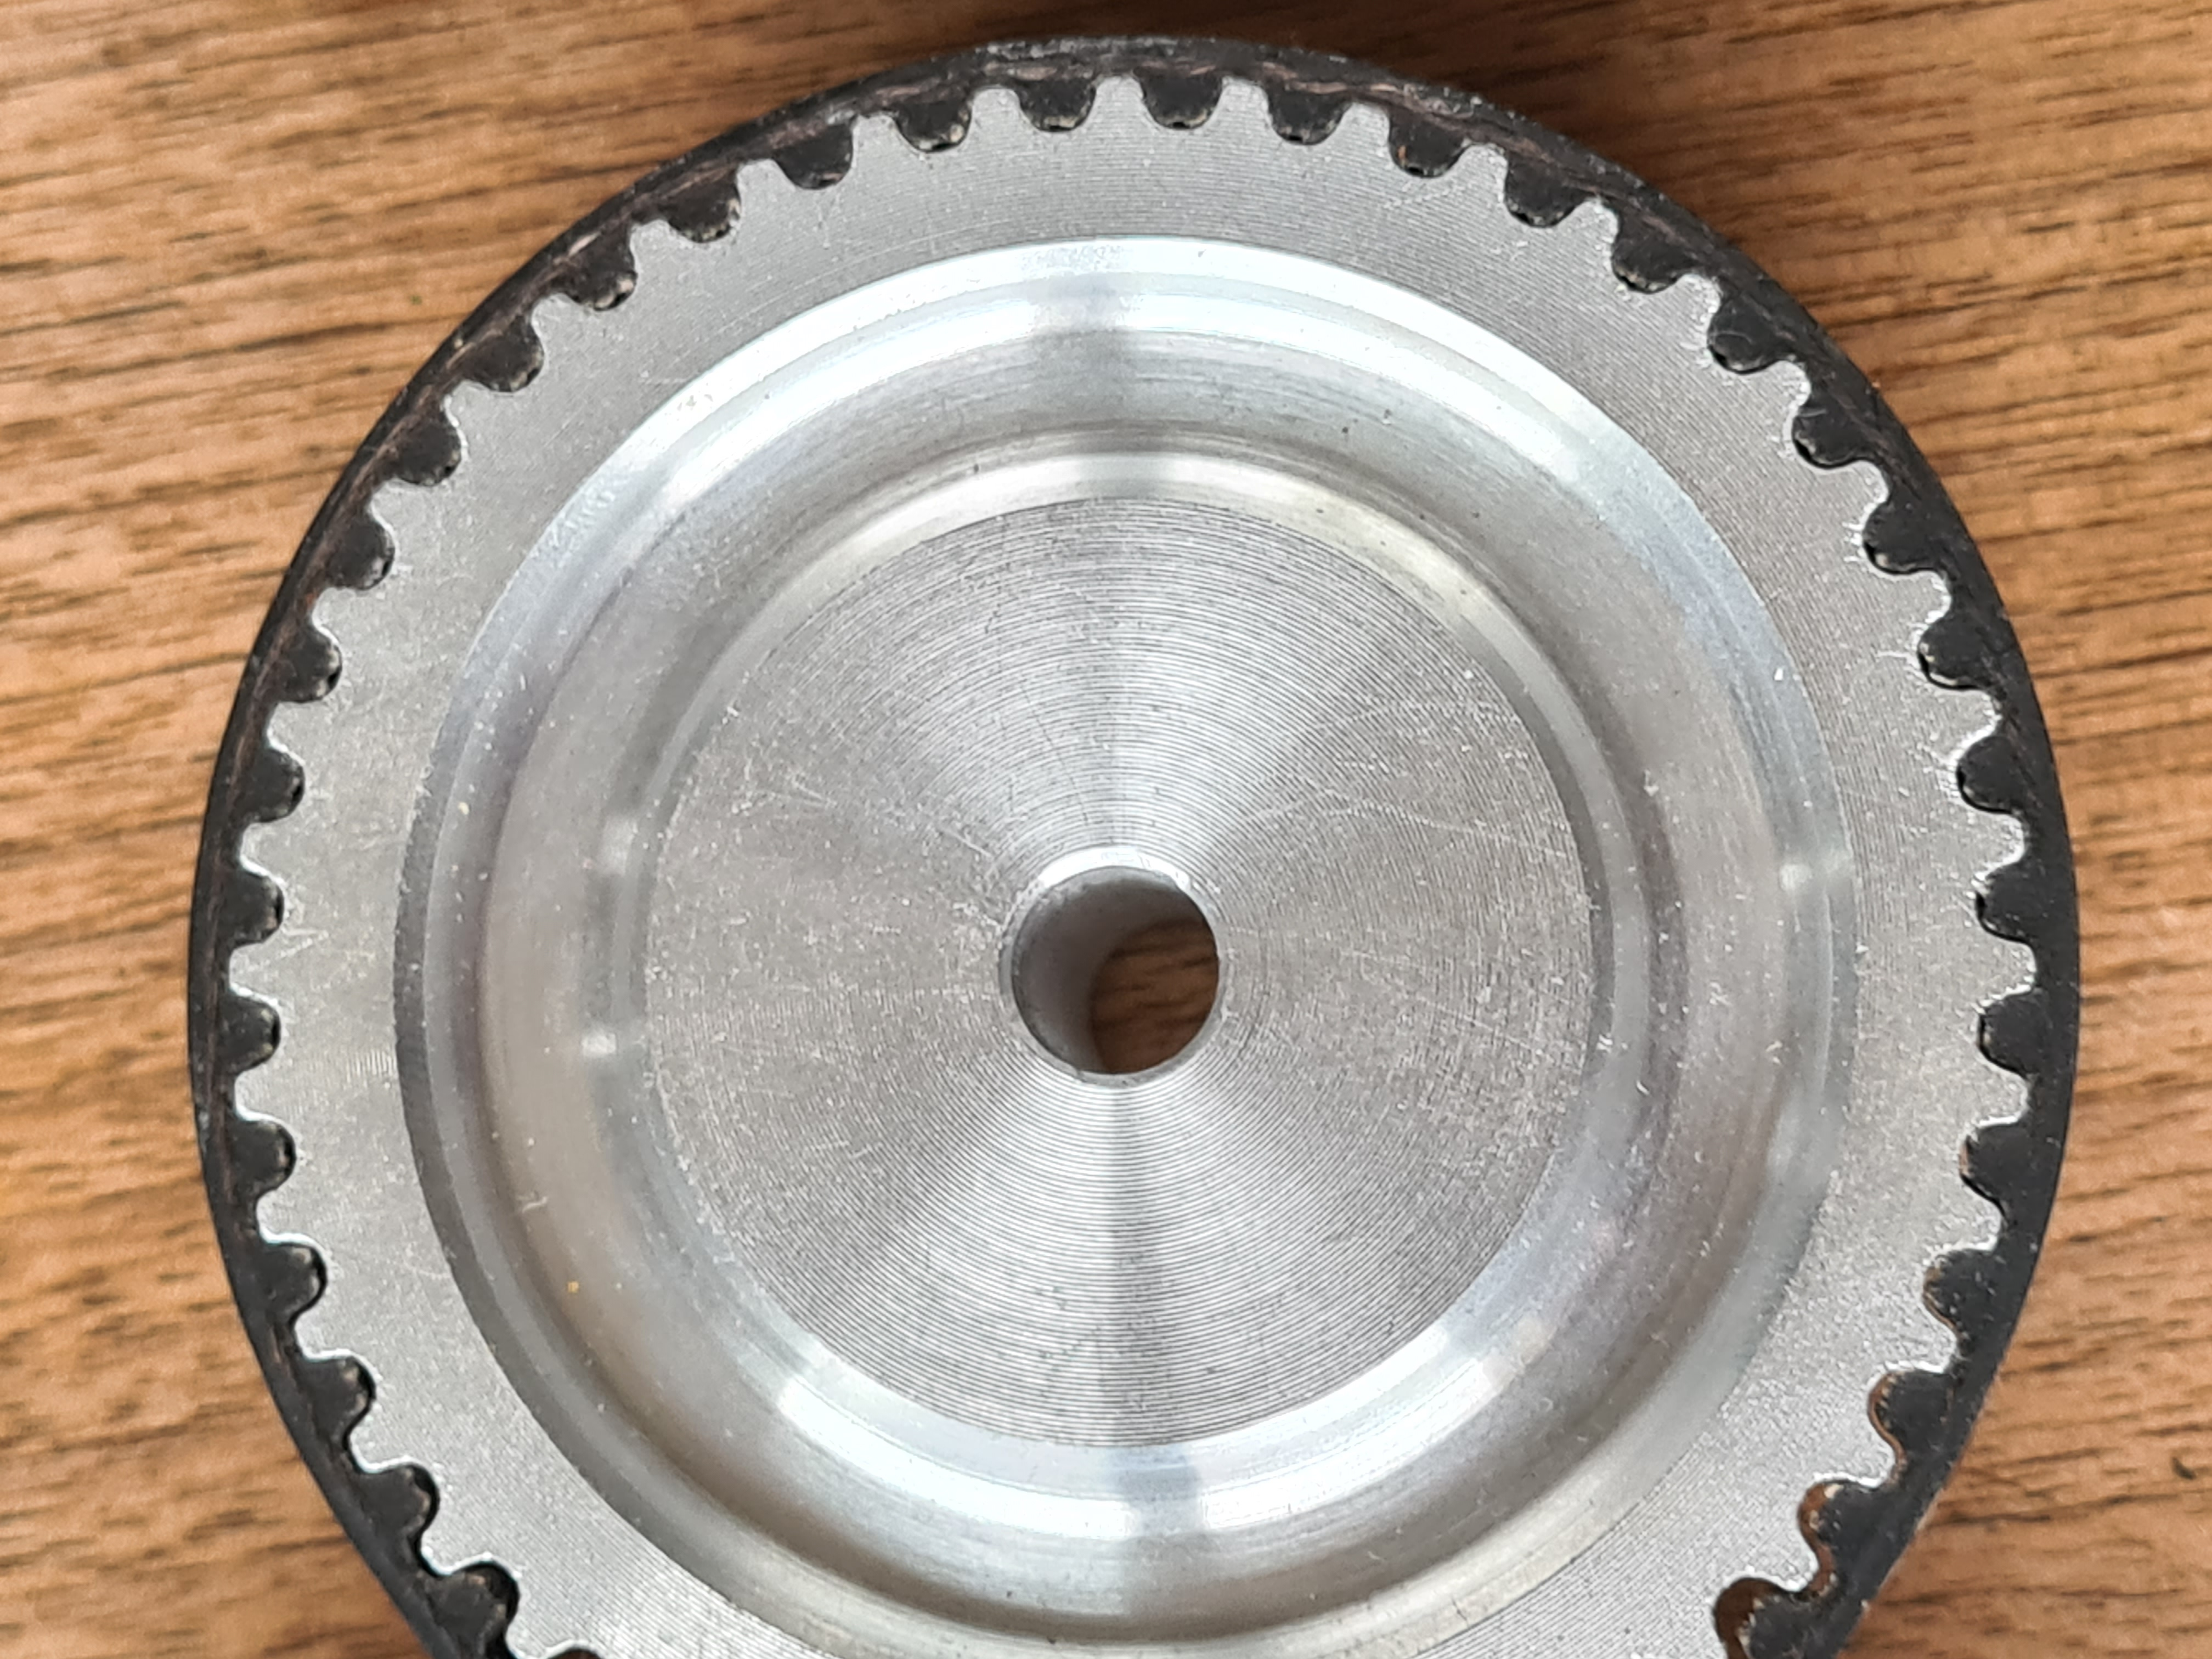
\includegraphics[width=\textwidth]{Footage/Pictures/Machined-HTD_tooth_fit.jpg}
				\caption{CNC-gefrästes HTD-5M-Profil auf Riemen.}%
				\label{subfig:machined HTD}
			\end{subfigure}
			\hfill
			\begin{subfigure}{.49\textwidth}
				\centering
				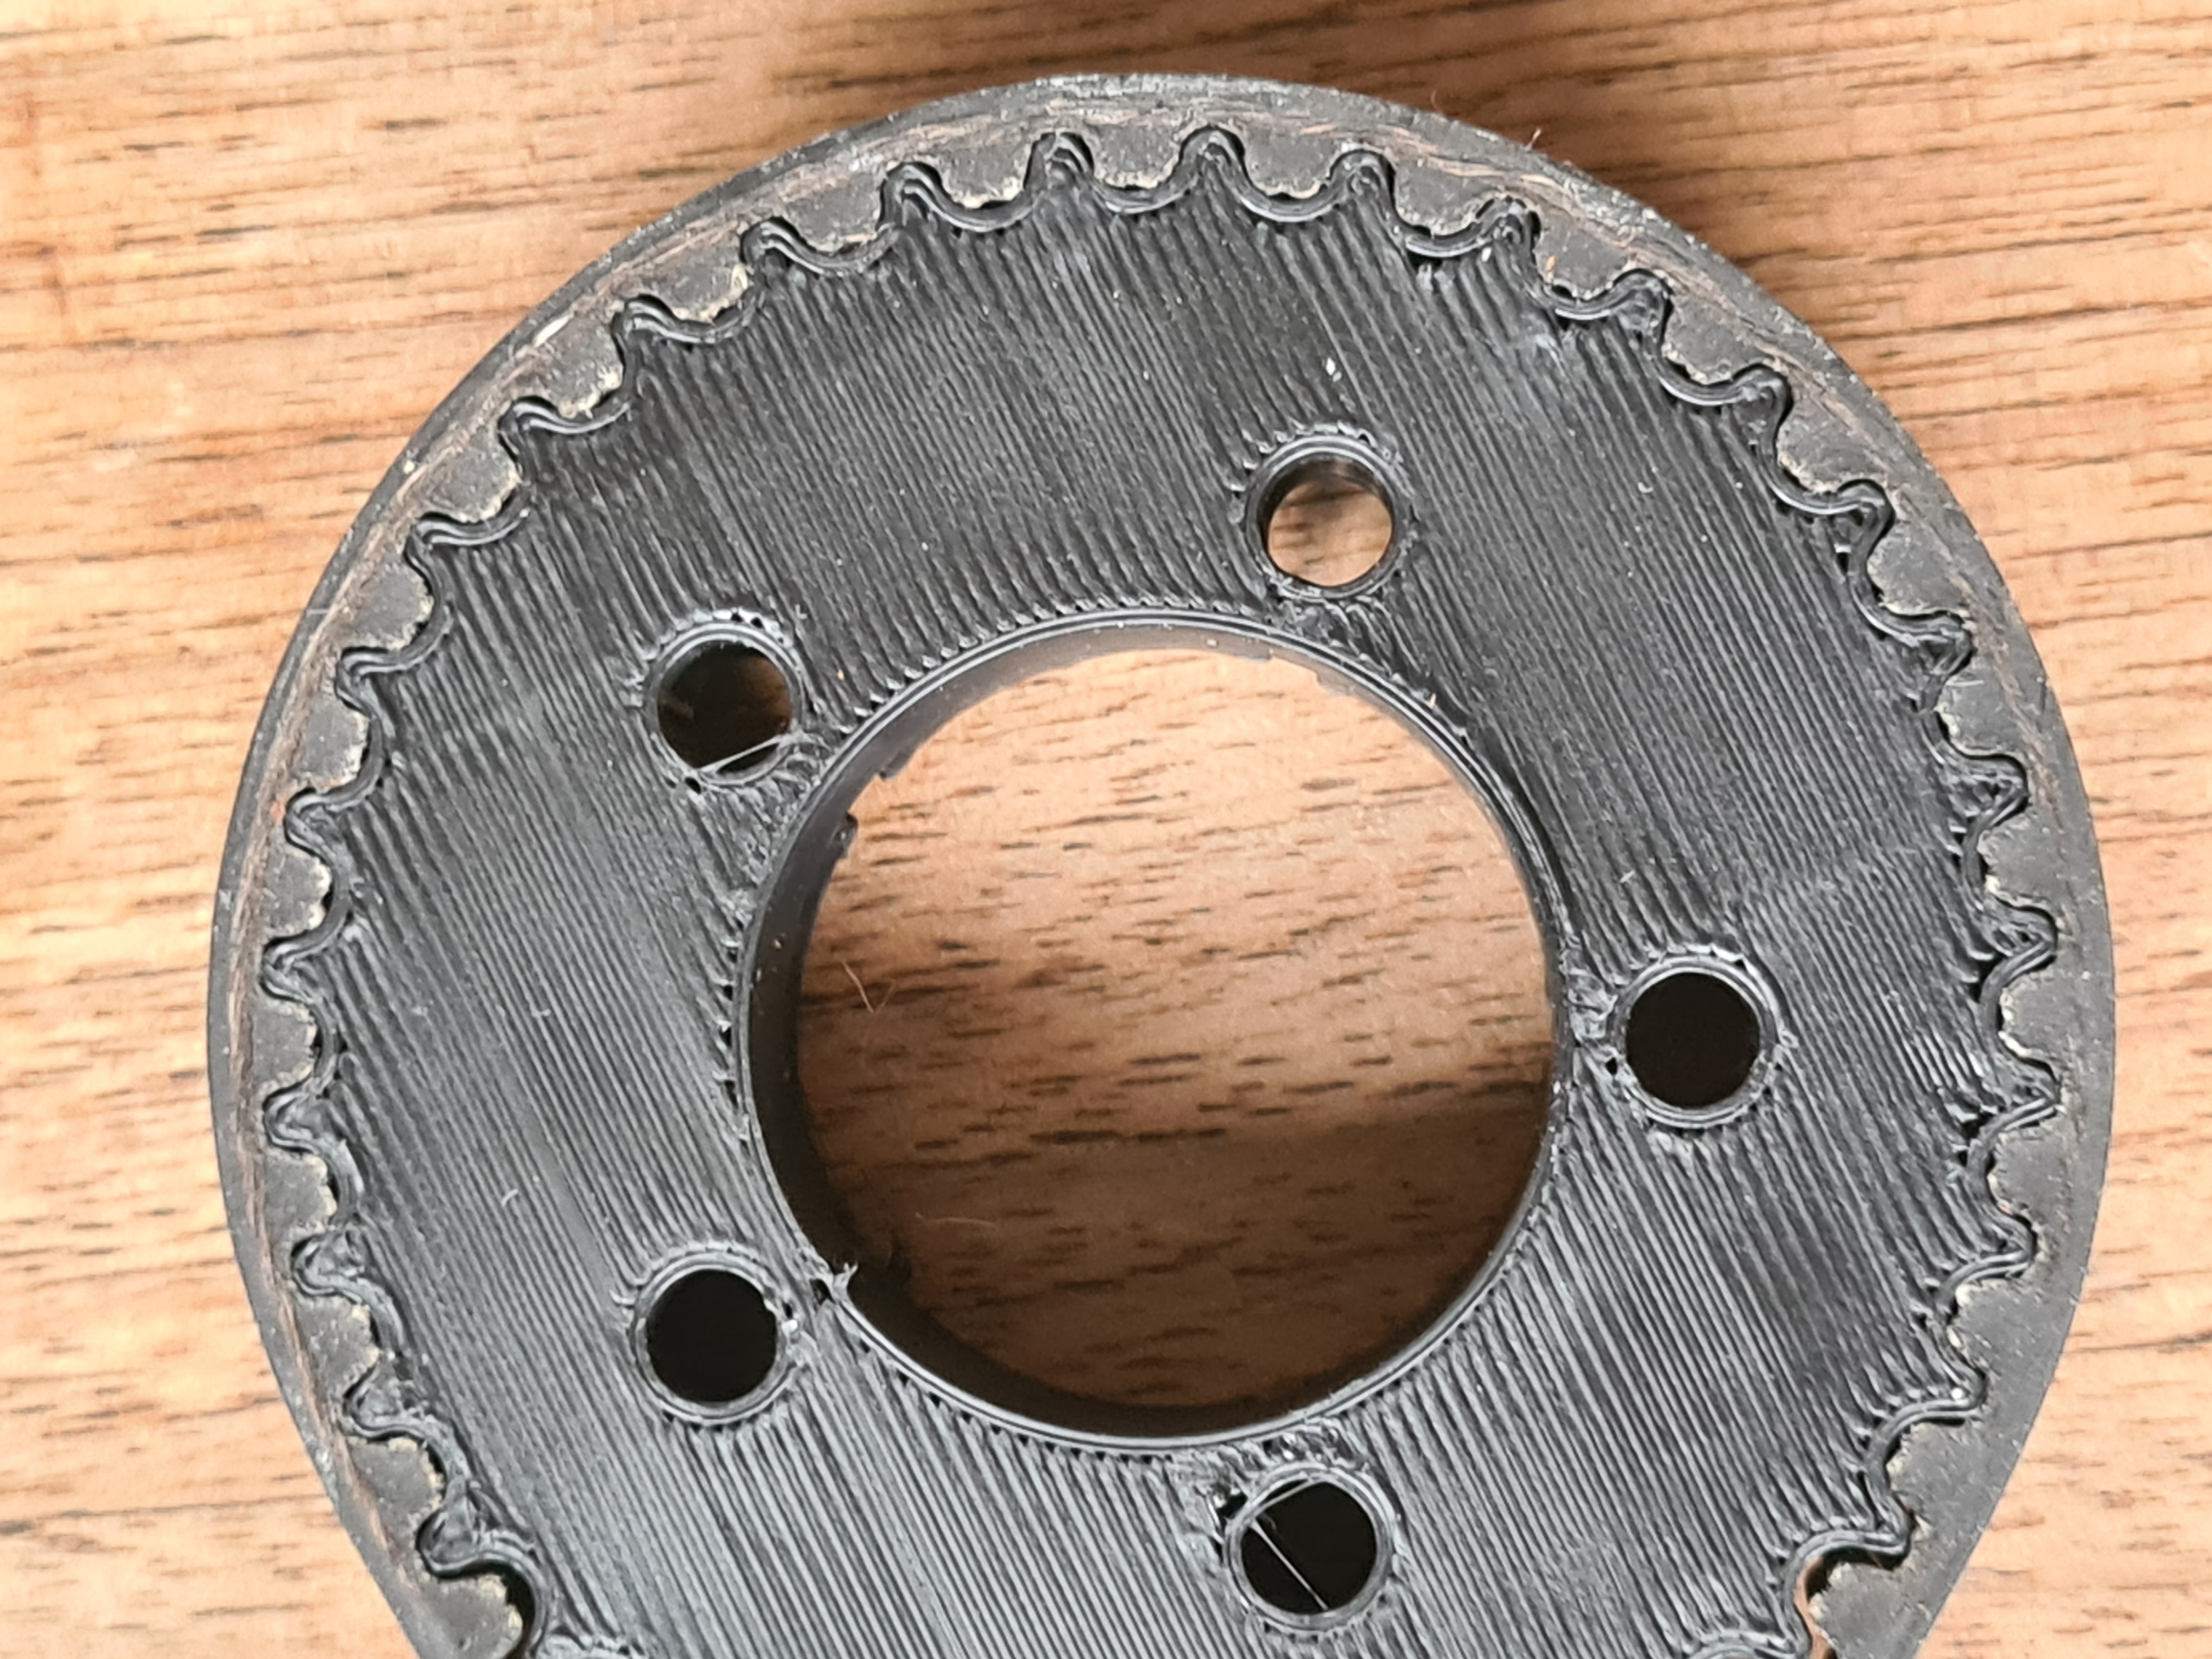
\includegraphics[width=\textwidth]{Footage/Pictures/Printed-HTD_tooth_fit.jpg}
				\caption{3D-gedrucktes HTD-5M-Profil auf Riemen.}%
				\label{subfig:printed HTD}
			\end{subfigure}
			\caption[Vergleich der Passform einer gekauften mit einer 3D-gedruckten Zahnriemenscheibe]{Vergleich der Passform einer gekauften Zahnriemenscheibe in (44T) aus Aluminium und des 3D-gedruckten Modells (36T) mit einem Riemen.}%
			\label{fig:HTD profiles comparison}
		\end{figure}\par\medskip
		%
		Da die Schrauben mit Muttern gekontert werden sollen und die der Zahnriemenscheibe gegenüberliegende Flanke der Rollen ebenfalls ein konkaves Profil aufweist, wurde ein komplementäres Gegenstück --~zu sehen in \cref{fig:orangatang kegel flat face} --~im oben beschriebenen Prozess modelliert.
		\begin{figure}[h]
			\centering
			\includesvg[width=.5\textwidth, inkscapelatex=false]{Footage/AwesomeBoard Transmission CAD/Drawings/Orangatang Kegel Flat Face}
			\caption[Zeichnung des Gegenstücks der Zahnriemenscheibe]{Zeichnung des Gegenstücks der Zahnriemenscheibe um eine ebene Fläche für die Muttern zur Verfügung zu stellen.}%
			\label{fig:orangatang kegel flat face}
		\end{figure}
		Wie auch die Zahnriemenscheibe enthält die Konterscheibe fünf Bohrungen und fünf Führungsstifte und soll ebenfalls möglichst exakt dem inneren Profil der Rollen anliegen.
		
		Aus Kostengründen und einfachem Zugang zu den Betriebsmitteln wurde entschieden, die funktionalen Versionen der getriebeseitigen Zahn- und Konterscheibe ebenfalls im 3D-Druck-Verfahren aus ABS selbst herzustellen.
		Es ist zwar zu erwarten, dass die Zahnriemenscheiben gegenüber aus Aluminium gefrästen Komponenten bezüglich Verschleiß und Festigkeit deutlich unterliegen, durch das gewählte Fertigungsverfahren lassen sich allerdings schnell, unkompliziert und günstig Ersatzteile herstellen.
		Darüber hinaus ist an dieser Stelle nicht mit einem plötzlichen Totalversagen der Materialintegrität und in Folge potenziell fataler Konsequenz zu rechnen.\par\medskip
		%
		Zur Auswahl des Riemens ist schließlich neben der Breite die Länge und damit die Anzahl der Zähne zu beachten.
		Ein vergrößerter Mittelpunktabstand beider Zahnriemenscheiben erhöht grundsätzlich die Anzahl greifender Zähne, allerdings fällt dieser Effekt mit zunehmendem Abstand schnell ab.
		Es wurde ein Abstand so gewählt, dass zu jeder Zeit ein Zahn mehr als gefordert greift.
		Mit Zahnungen von 36T für die Antriebsseite, 15T getriebeseitig und dieser Vorgabe wurde eine Riemenzahnung von 55T gewählt.
		Die Riemenbreite wurde mit \qty{12}{\milli\metre} arbiträr auf das breiteste käuflich erhältliche Maß festgelegt, dass noch konstruktiv umsetzbar ist.
		\Cref{fig:timing belt length} zeigt schematisch das System beider Zahnriemenscheiben und Riemen.
		\begin{figure}[h]
			\centering
			\includesvg[width=.8\textwidth, inkscapelatex=false]{Footage/AwesomeBoard Transmission CAD/Drawings/Timing Belt assembly}
			\caption[Mittelpunktabstand zwischen antriebs- und getriebeseitigen Zahnriemenscheiben]{Mittelpunktabstand zwischen antriebs- und getriebeseitigen Zahnriemenscheiben bei einem Zahnriemen mit 55 Zähnen.}%
			\label{fig:timing belt length}
		\end{figure}
	\section{Motorbefestigung}\label{sec:motorbefestigung}
		Die Verbindung zwischen Motor und Hanger wird in zwei Teilen hergestellt: eine Zange, die formschlüssig Verdrehen um die Hangerachse und durch Verspannen reibschlüssig Verschieben entlang der Hangerachse verhindert und ein Arm, der die Verbindung zwischen Zange und Motor herstellt.
		Kostenfreie Verfügbarkeit des Materials lässt die Werkstoffauswahl beider Komponenten auf Walzbleche der Aluminiumlegierung AlMgSi0,5 (EN AW 6060) fallen.
		Die Fertigung findet im CNC-Fräsverfahren mit einem Werkzeugdurchmesser von \qty{3}{\milli\metre} statt.

		\begin{figure}[h]
			\centering
			\includesvg[width=.6\textwidth, inkscapelatex=false]{Footage/AwesomeBoard Transmission CAD/Drawings/Mount - Hanger Clamp}
			\caption[Zange zur Montage der Motorhalterung am Hanger]{Zange zur Montage der Motorhalterung am Hanger.}%
			\label{fig:hanger clamp drawing}
		\end{figure}
		\Cref{fig:hanger clamp drawing} zeigt eine Zeichnung der Zange mit allen relevanten Dimensionen.
		Erkennbar ist mittig eine Aussparung in Form des Profils des \textit{Caliber II} Hangers mit Nut, um durch eine M5 Schraube an den beiden flachen Flanken des Hanger angespannt werden zu können.
		Um hier die Kontaktfläche zu maximieren wurde als Halbzeug ein Blech größtmöglich zur Verfügung stehender Materialstärke gewählt.
		Kreisförmig um die Rollachse des Hangers befinden sich sechs M4-Durchgangsbohrungen, um flach anliegend den Motorarm anbringen zu können.
		Sollte die Einspannung des Hangers in der Zange ein Driften entlang der bzw. Kippen gegen die Hangerachse nicht zuverlässig verhindern können, so sollen später an den drei Aussparungen entlang des äußeren Bogens Querverbindungen zwischen zwei gegenüberliegenden Zangen möglich sein.
		\begin{figure}[h]
			\centering
			\includesvg[width=.7\textwidth, inkscapelatex=false]{Footage/AwesomeBoard Transmission CAD/Drawings/Mount - Motor Piece}
			\caption[Verbindungsarm zwischen Motor und Hangerzange]{Verbindungsarm zwischen Motor und Hangerzange. Wichtigste Merkmale: links radial um die Rollachse angeordnete Langlöcher zur Feinjustage des Montagewinkels. Rechts entlang der Längsachse des Armes ausgerichtete Langlöcher zur Justage der Riemenspannung.}%
			\label{fig:motor piece drawing}
		\end{figure}

		Ebenfalls aus AlMgSi0,5 und mit einer Materialstärke von \qty{4}{\milli\metre} stellt der Arm als komplementäre Komponente, flach an die Zange angeschraubt, eine steife Verbindung zwischen Hanger und Motor her.
		In \cref{fig:motor piece drawing} links befinden sich radial um die Rollachse angeordnet sechs Langlöcher zur Montage an der Zange.
		Da der gesamte Aufbau sich unterhalb des Decks befinden wird, ist es wichtig bezüglich der Motoren ein Optimum zwischen Bodenabstand und Distanz zum Deck zu finden.
		Um auch nach Zusammenbau die Abstände nachjustieren zu können, kann der Anstellwinkel des Armes innerhalb eines Winkels von \qty{22,5}{\degree} so auf einfache Weise angepasst werden.
		\begin{figure}[h]
			\centering
			\includesvg[width=.75\textwidth, inkscapelatex=false]{Footage/AwesomeBoard Transmission CAD/Drawings/Drivetrain inclined}
			\caption[Zeichnung des Gesamtaufbaus]{Zeichnung des Gesamtaufbaus montiert als Hinterachse.}
			\label{fig:drivetrain inclined}
		\end{figure}
		Rechts befinden sich vier weitere Langlöcher von \qty{6}{\milli\metre} Länge zur Befestigung des Motors.
		Hier dienen die Langlöcher der Möglichkeit nach Zusammenbau durch Variation des Abstandes von Roll- zu Motorachse die Riemenspannung nachjustieren zu können.
		Nach \cref{fig:timing belt length} ist mit der in \cref{sec:transmission} beschriebenen Konfiguration ein theoretischer Mittelpunktabstand von \(\approx \qty{74,34}{\milli\metre}\) zu erwarten.
		Der Mittelpunktabstand der Hangerachse und des Kreismittelpunktes der Langlöcher zur Motorbefestigung wurde mit \qty{73,5}{\milli\metre} so gewählt, dass bei einer Länge der Langlöcher von \qty{6}{\milli\metre} sowohl Ein- und Ausbau des Riemens, als auch adäquate Riemenspannung sichergestellt ist.

		Vier Bohrungen durch die äußeren Erhebungen um die Motorachse herum sollen es später ermöglichen bei Bedarf einen Riemenschutz anbringen zu können.
		Die Erhebungen selbst sollen den Zweck eines Puffermaterial im Falle eines Bodenkontaktes erfüllen.
		\begin{figure}[h]
			\centering
			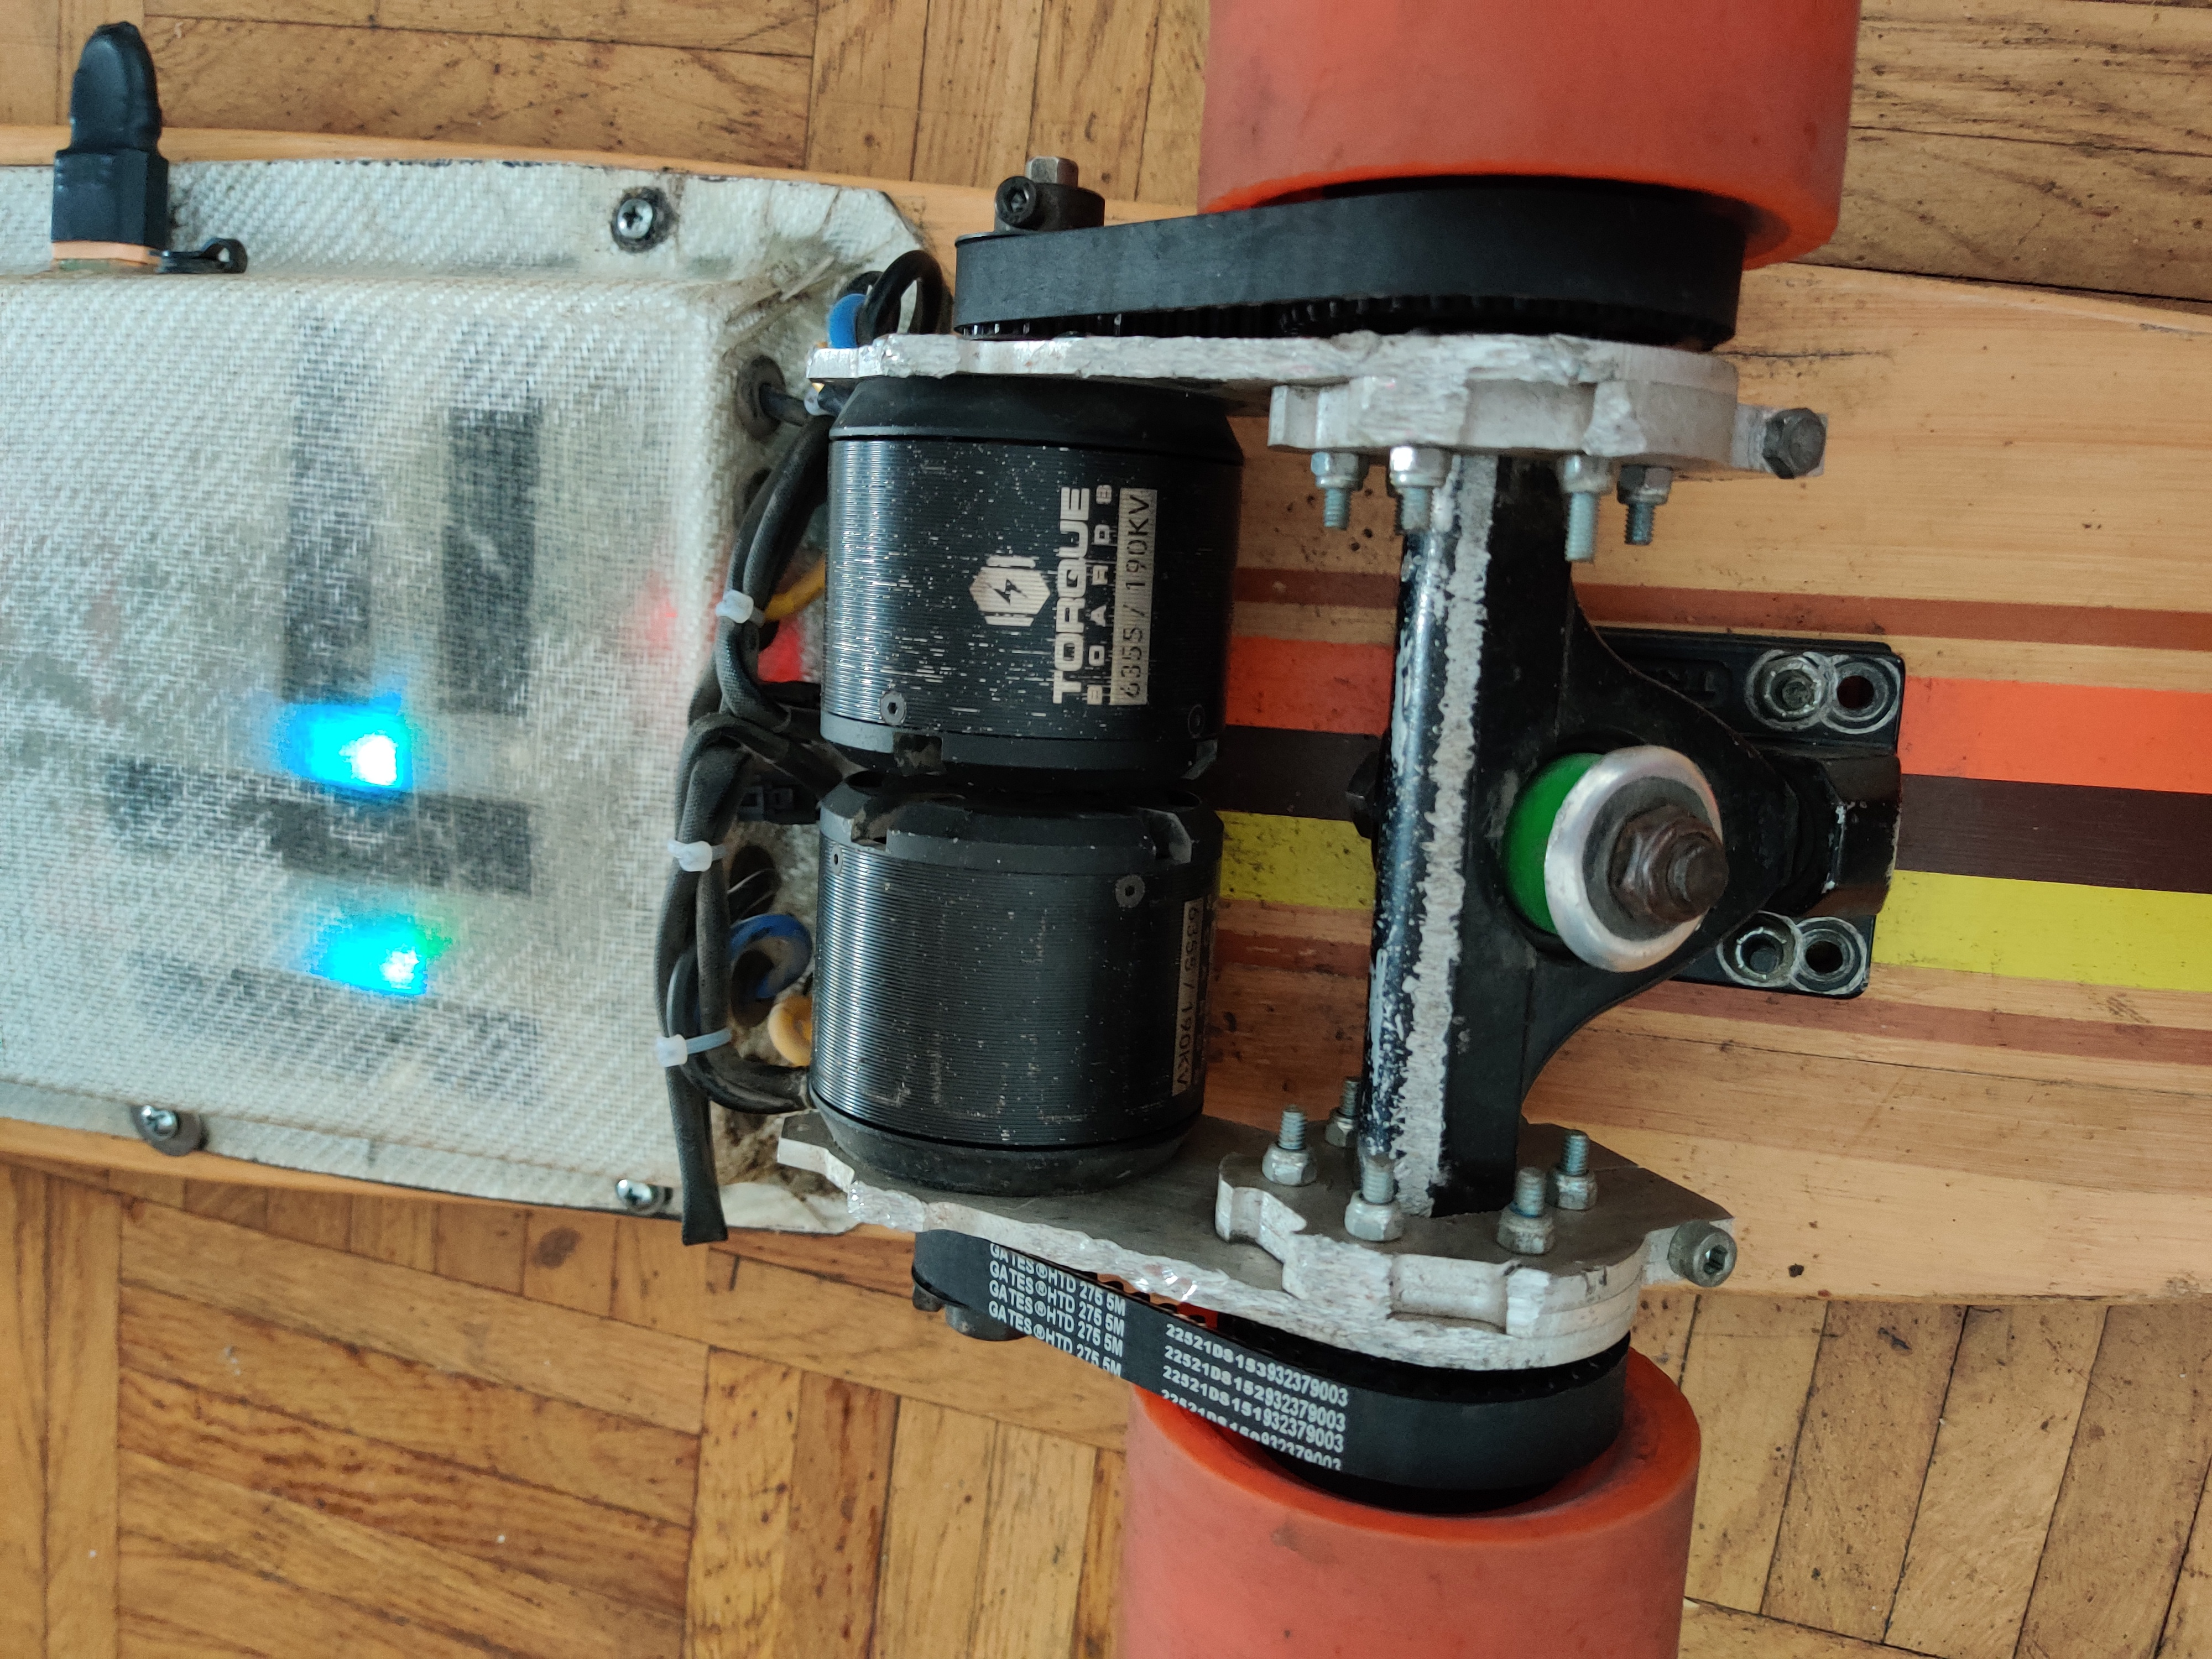
\includegraphics[angle=180, width=.5\textwidth]{Footage/Pictures/Drivetrain close up v2.jpg}
			\caption[Fertiger Aufbau des Antriebssystems]{Fertiger Aufbau des Antriebssystems nach etwa~\qty{100}{\kilo\metre} Testfahrt durch urbanes Terrain.}
			\label{fig:real world assembly}
		\end{figure}

		\Cref{fig:drivetrain inclined} zeigt eine Zeichnung des Gesamtaufbaus des Systems mit zwei Motoren, den Unterbaugruppen der Motorhalterungen, den Rollen und den Truck montiert an der Heckseite des Decks in eingelenkter Position.
		Zum Vergleich in \cref{fig:real world assembly} der reale Aufbau.
% LTeX: language=de-DE
\chapter{Elektronik}
	Die verwendeten ESC sind in der Lage die rückwirkende elektromotirische Kraft (rEMK\nomenclature[A]{rEMK}{Rückwirkende elektromotorische Kraft}) --~eine während des Betriebes in den Wicklungen des Motors erzeugte und seiner Drehrichtung entgegenwirkenden Spannung -- zu Messen und zur Positionsbestimmung des Rotors zu nutzen.
	Gegenüber eines trapezoidalen Phasenstromes können die Motorwicklungen so sinusoidal bestromt werden, was wiederum geringere elektrische Verluste und ein gleichmäßigeres Drehmomentprofil während eines Umlaufes und damit einen sanfteren und geräuschärmeren Motorlauf verspricht.
	Prinzipbedingt steigt die Amplitude der rEMK mit der Drehzahl des Motors.
	Konsequenterweise wird so die Messung und damit die Positionsbestimmung im niedrigen Drehzahlbereich erschwert während sie im Stillstand unmöglich wird.
	Um ein exaktes Feedback der Rotorposition an die Steuerelektronik unabhängig der rEMK zu ermöglichen, verfügen die ausgewählten Motoren über integrierte Hall-Effekt-Sensoren.
	Im höheren Drehzahlbereich verschwinden ihre Vorteile zwar zunehmend, liefern jedoch die Möglichkeit eines äußerst sanften Anlaufes aus dem Stillstand heraus.\par\medskip
	%
	\begin{wrapfigure}{r}{.5\textwidth}
		\centering
		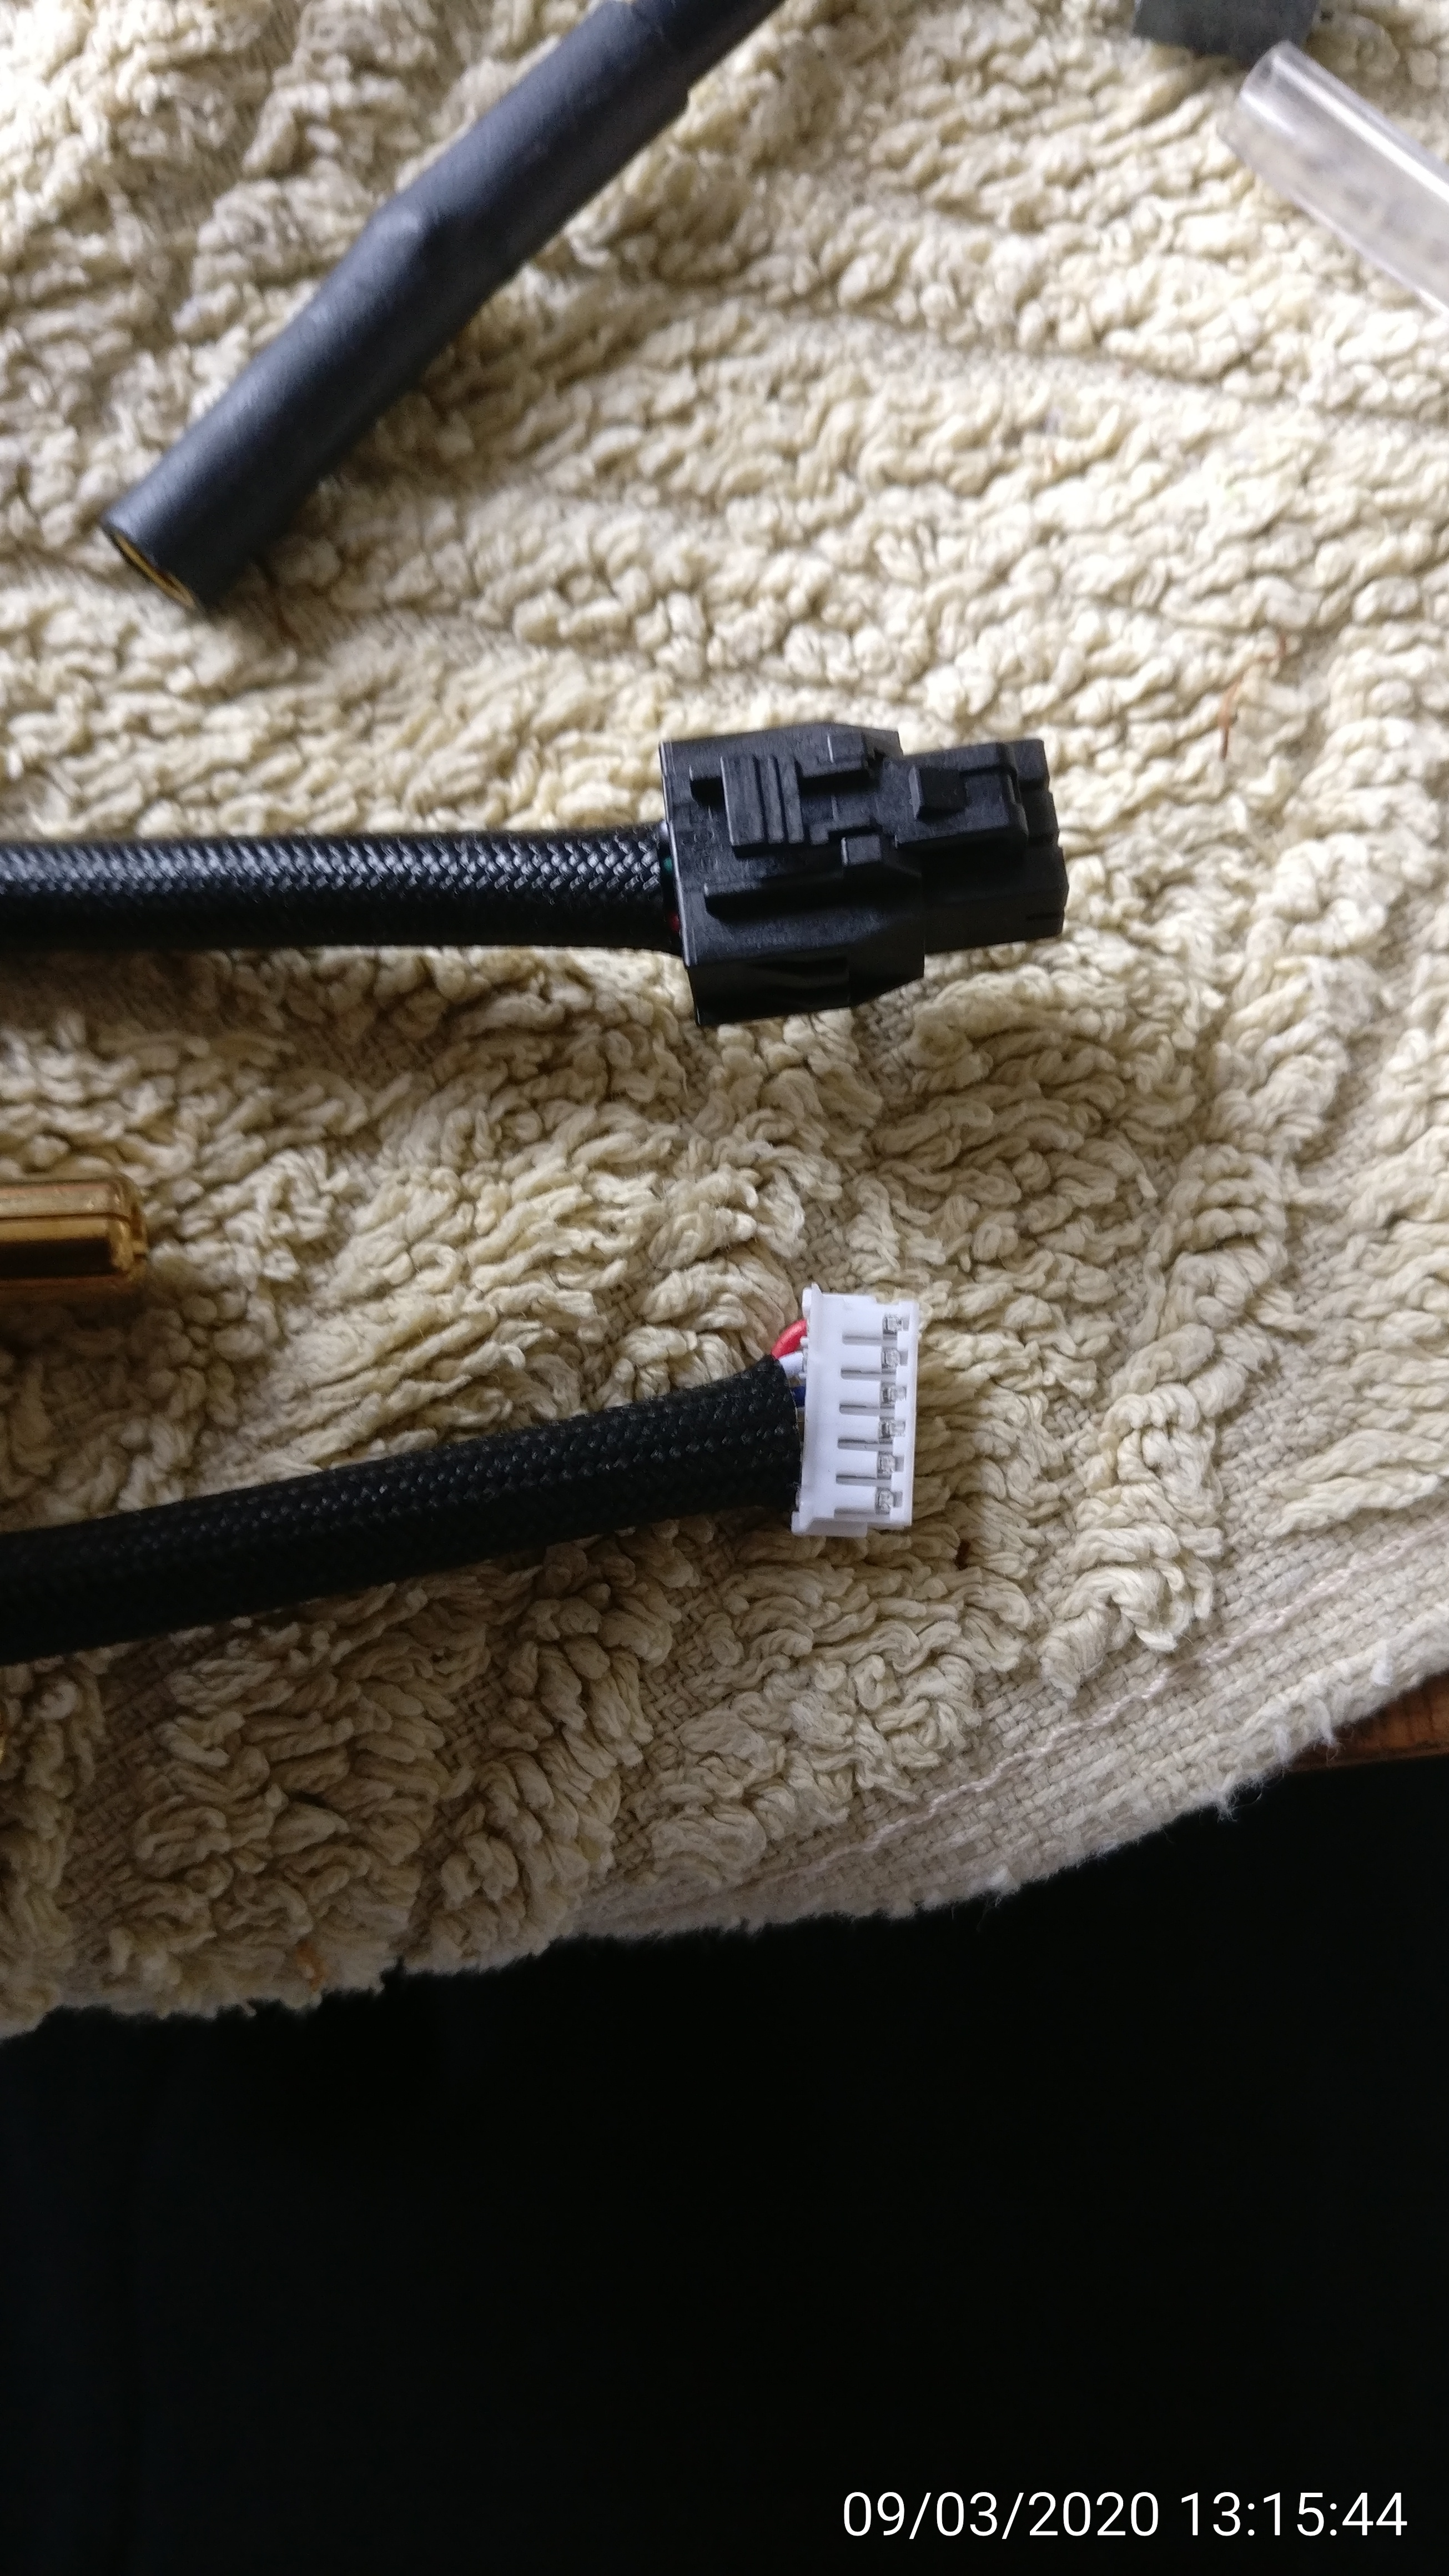
\includegraphics[angle=90, width=.4\textwidth]{Footage/Pictures/Hall sensor connector.jpg}
		\caption[Hall-Sensoren Konnektoren]{Links ein 3x2-Pin Molex Micro-Fit 3.0 Konnektor, rechts ein 6-Pin JST-PH zur Verbindung mit dem ESC.}
		\label{fig:hall sensor connectors}
	\end{wrapfigure}
	Die ab Werk unterminierten Sensorenleitungen wurden im Sinne einer Staub- und Spritzwassergeschützen Durchführung in das GFK-Gehäuse über eine Kabelbrücke mit den ESC verbunden.
	Die Kabelbrücke wurde aus 30AWG\nomenclature[A]{AWG}{American Wire Gauge}\footnote{Entspricht etwa \qty{0,25}{\milli\metre\squared}.} flexibler Silikonleitung mit einem 6-Pin JST-PH Konnektor ESC-seitig und einem 3x2 Molex Micro-Fit 3.0 Konnektor motorseitig gefertigt (vgl. \cref{fig:hall sensor connectors}).
	Für den motorseitigen Anschluss wurde eine entsprechende Öffnung in das Gehäuse geschnitten und der Konnektor mit Epoxidharz dauerhaft und dicht verbunden.
	Die Anordnung der Sensoren spielt an dieser Stelle eine untergeordnete Rolle, da sie vor Inbetriebnahme softwareseitig konfiguriert werden können.
	Es wird lediglich darauf geachtet, dass die Anordnung beider Motoren identisch bleibt.
	Zur Durchführung der Phasenleitungen werden je Motor drei Löcher in das Gehäuse gebohrt und mit Gummiösen versehen.\par\medskip
	%
	Die hardwareseitige Leistungsendstufe ist als Doppel-H-Brücke implementiert und in \cref{fig:power mosfets} gezeigt.
	Um den Rotor um einen Winkel \qty{360}{\degree} dividiert durch die Anzahl der Polpaare \(n_\text{p}\)\nomenclature[L]{\(n_\text{p}\)}{Anzahl der Polpaare\nomunit{1}} zu drehen, muss ein voller Kommutationszyklus durchgeführt werden, was im Folgenden einer elektrischen Umdrehung entsprechen soll.
	Die Anzahl elektrischer Umdrehungen je Minute bei gegebener mechanischer Drehzahl des Rotors sei somit gegeben durch:
	\begin{align}
		ERPM = \omega \cdot n_\text{p}
		\label{eq:ERPM and RPM}
	\end{align}
	Die Maximalgeschwindigkeit skaliert somit direkt proportional mit \(ERPM\) nach
	\begin{align}
		v_\text{max} = \frac{ERPM \cdot 2\pi \cdot r}{n_\text{p} \cdot \zeta}
		\label{eq:max speed by ERPM}
	\end{align}
	Die Konfigurationssoftware der ESC lässt zu, dass ein oberer Grenzwert für \(ERPM\) und damit unmittelbar für die Maximalgeschwindigkeit definiert werden kann.

	% Die technische Dokumentation der ESC empfiehlt, \(ERPM\) unterhalb eines Wertes von \num{60000} zu halten.

	% Bei gegebener Batteriespannung und den verwendeten Motoren mit sieben Polpaaren liefert \cref{eq:max rpm} multipliziert mit dem zweifachen der Polpaarzahl ein theoretisches Maximum der ERPM von \num{95760} und liegt damit deutlich über dem empfohlenen oberen Grenzwert.
	% Die ESC verfügen über die Möglichkeit, hier softwareseitig Maximal- und Minimalwerte zu hinterlegen.
	% Mit zusätzlichem Sicherheitsabstand von \qty{10}{\percent} wird ein oberer Grenzwert von \num{54000} festgelegt was einer reduzierten Maximalgeschwindigkeit von etwa \qty{24}{\kilo\metre\per\hour} entspricht.
% LTeX: language=de-DE
\chapter{Evaluation}
	Im Folgenden sollen die mechanische Integrität und Performanz des Systems mit Respekt auf die in \cref{sec:constructive limitations} formulierten Rahmenbedingungen diskutiert werden.
	Im Vorfeld wurden mehrere Testfahrten auf urbanem Untergrund und entlang verschiedener Steigungen durchgeführt.
	Insgesamt wurde die verbaute Batterie hierbei dreimal von~\qty{42}{\volt} (voll geladen) herunter auf~\qty{31}{\volt} entladen.
	Zurückgelegte Distanz und mittlere, sowie maximale Geschwindigkeit wurden mittels Navigationssoftware und GPS gemessen.
	Zusätzlich wurden Logginginformationen der ESC selbst zur Evaluation herangezogen.
	% \Cref{fig:ESC plot} zeigt den Verlauf der Geschwindigkeit in~\unit{\kilo\metre\per\hour} zusammen mit Motor- und Batteriestrom in~\unit{\percent} der jeweiligen Maximalwerte.
	Die verwendeten Parameter für Tests auf der Werkbank und im Feld können \cref{fig:ESC motor params} und \cref{fig:ESC erpm setting} entnommen werden.
	% Da aus Sicherheitsgründen einige Testläufe auf der Werkbank durchgeführt wurden und Messungen per GPS jedoch eine tatsächliche Bewegung im freien zwingend erforderlich machen, wurden zusätzlich Logginginformationen der ESC ausgelesen, um aus Umdrehungen pro Minute und Anzahl der Umdrehungen Werte zur Geschwindigkeit rechnerisch ermitteln zu können.\par\medskip
	%

	\begin{figure}[h]
		\centering
		\includesvg[width=.75\textwidth, inkscapelatex=false]{Footage/AwesomeBoard Transmission CAD/Drawings/Drivetrain inclined}
		\caption[Zeichnung des Gesamtaufbaus]{Zeichnung des Gesamtaufbaus montiert als Hinterachse.}
		\label{fig:drivetrain inclined}
	\end{figure}

	\Cref{fig:drivetrain inclined} zeigt eine Zeichnung des Gesamtaufbaus des Systems mit zwei Motoren, den Unterbaugruppen der Motorhalterungen, den Rollen und den Truck montiert an der Heckseite des Decks in eingelenkter Position.
	Zum Vergleich in \cref{fig:real world assembly} der reale Aufbau.
	\begin{figure}[h]
		\centering
		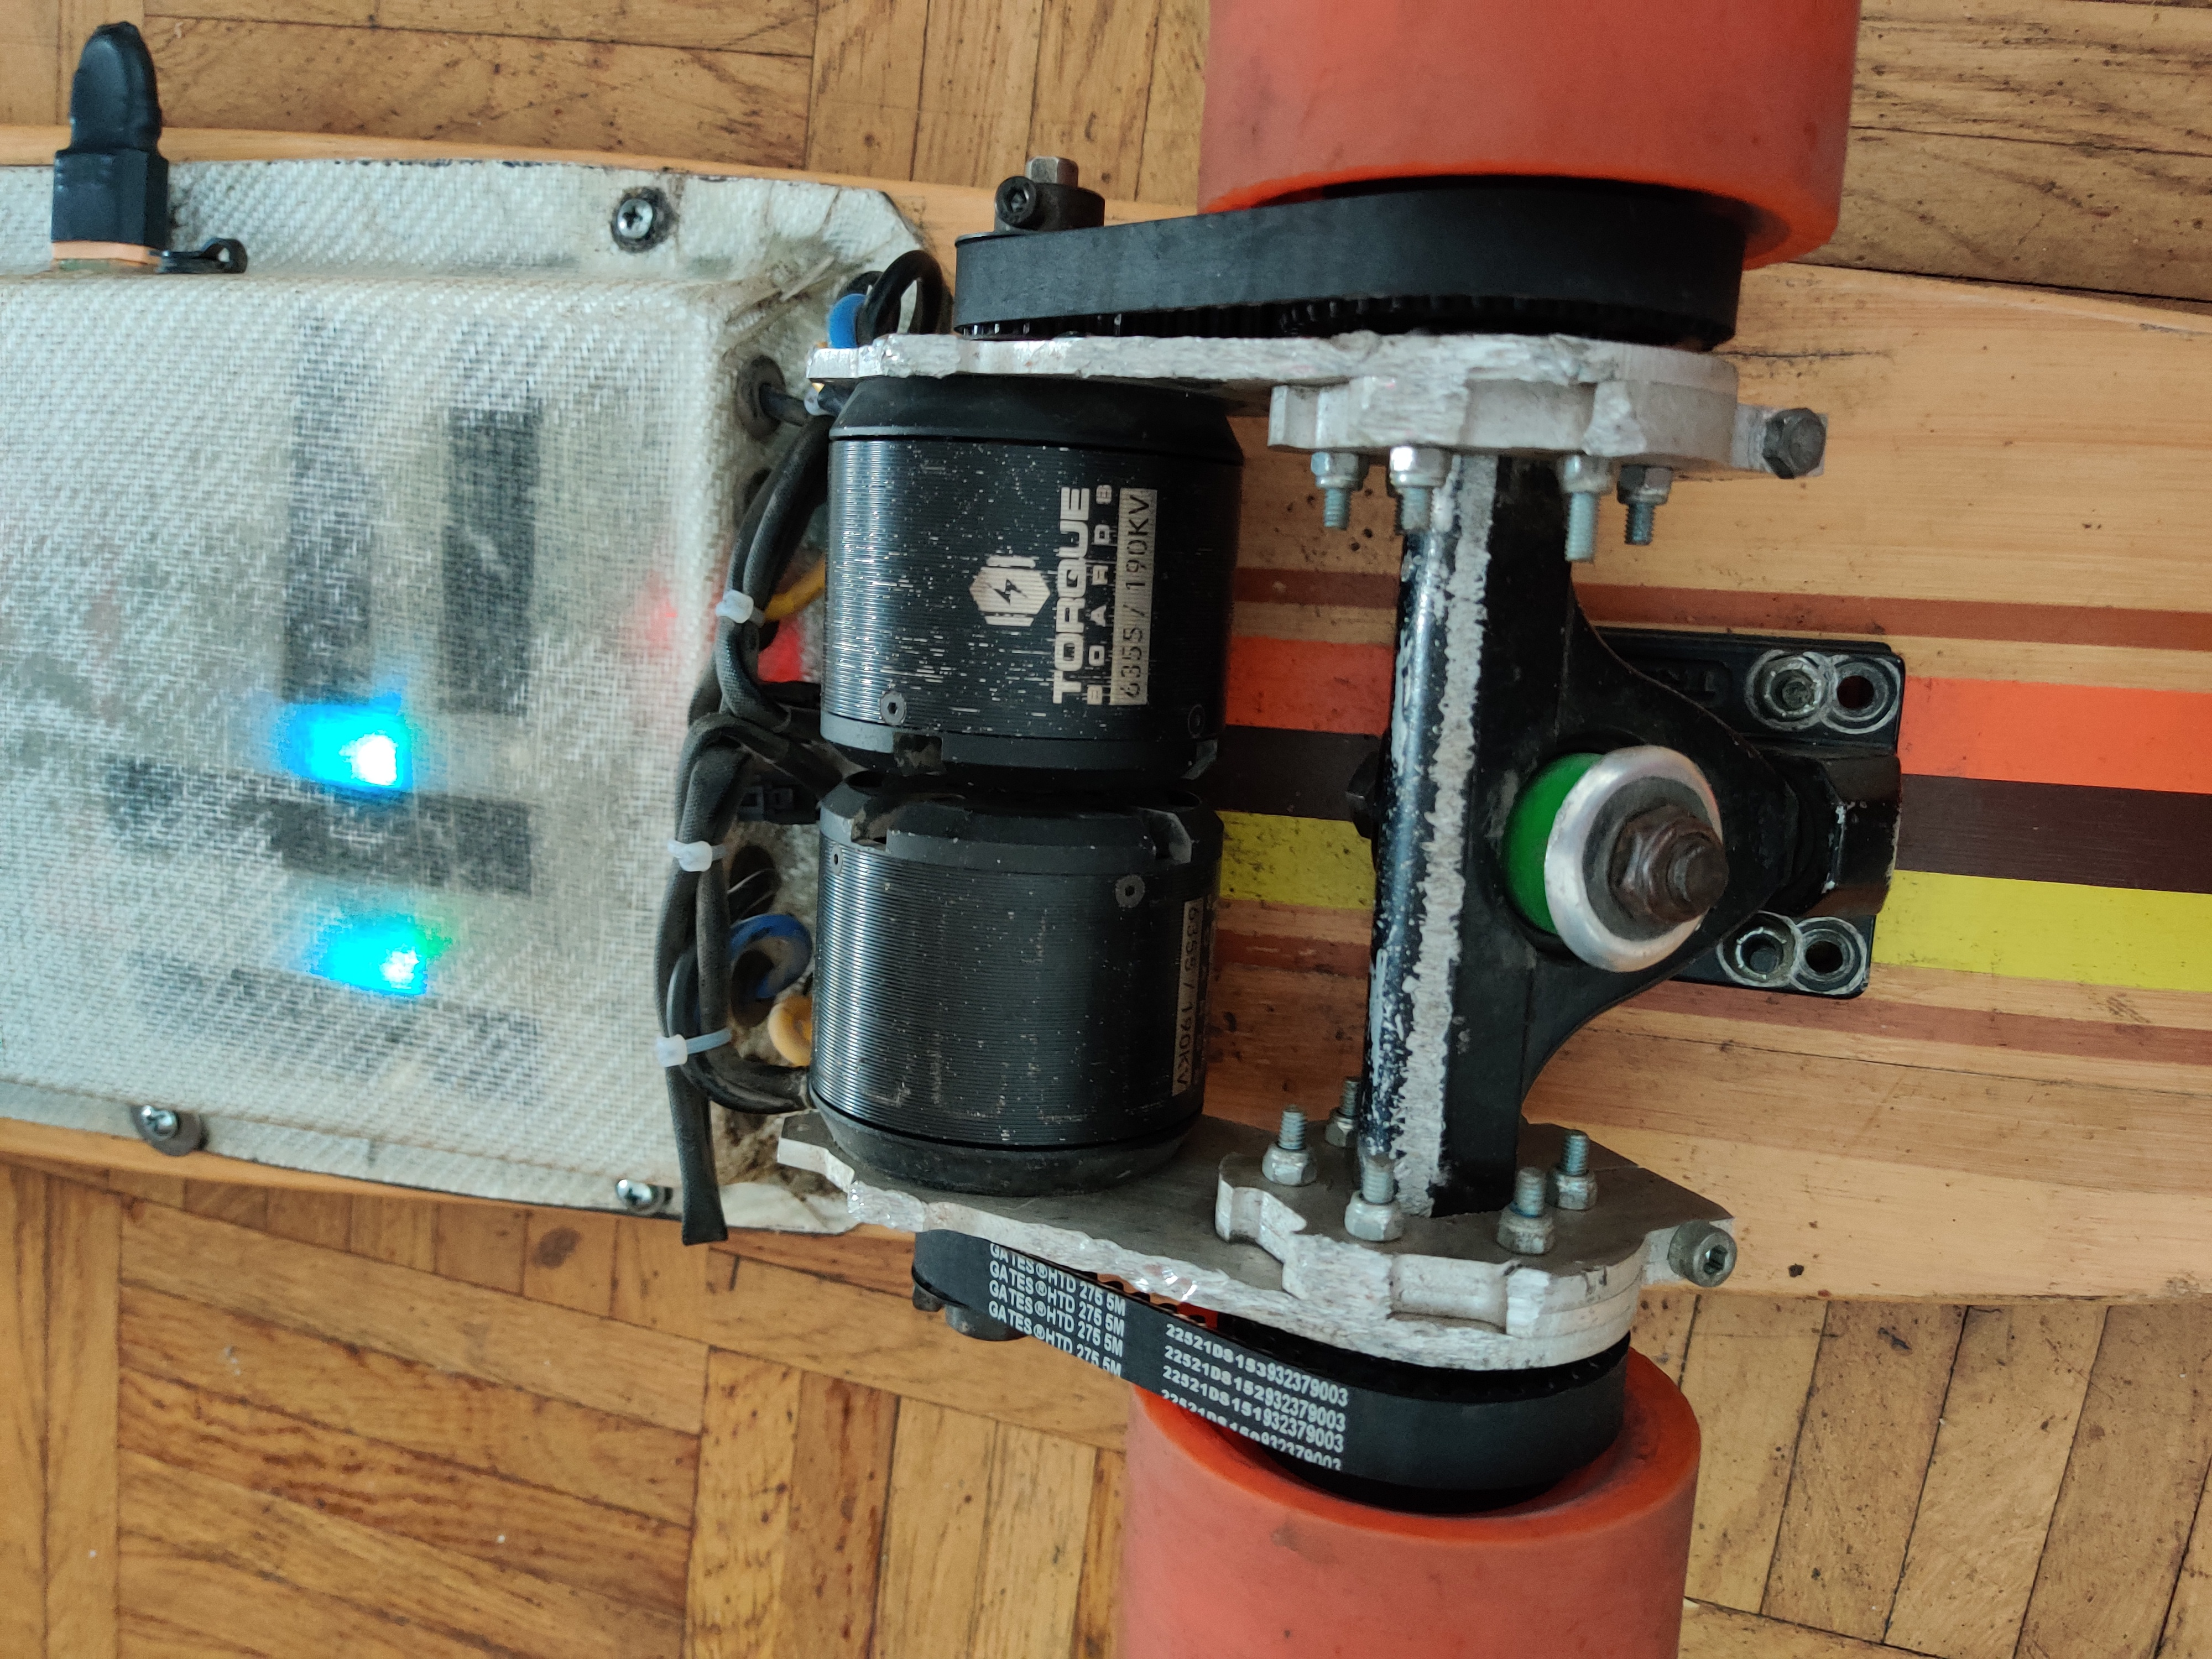
\includegraphics[angle=180, width=.5\textwidth]{Footage/Pictures/Drivetrain close up v2.jpg}
		\caption[Fertiger Aufbau des Antriebssystems]{Fertiger Aufbau des Antriebssystems nach etwa~\qty{100}{\kilo\metre} Testfahrt durch urbanes Terrain.}
		\label{fig:real world assembly}
	\end{figure}
	%
	\section{Performanz}
		Während mehrerer Testfahrten wurde das Drehmoment auf einer Strecke von etwa~\qty{250}{\metre} entlang eines Hanges mit einer maximalen Steigung von~\qty{7,5}{\percent} auf gepflastertem Untergrund getestet.
		Während das System am Hang und aus dem Stand heraus nur schwer in der Lage ist zu beschleunigen, ist es ohne weiteres möglich mit bereits moderater Anfangsgeschwindigkeit die Steigung zu überwinden.
		% \begin{figure}[h]
		% 	\centering
		% 	\includesvg[width=.85\textwidth, inkscapelatex=false]{Calc/ESC_plot}
		% 	\caption[ESC plot]{ESC plot.}%
		% 	\label{fig:ESC plot}
		% \end{figure}
		\begin{figure}[h]
			\centering
			\includesvg[width=\textwidth]{Calc/ESC_testdrive_plot}
			\caption[Aufgetragene Logging-Informationen einer Testfahrt]{Aufgetragene Logging-Informationen einer Testfahrt von etwa~\qty{2,8}{\kilo\metre}. Oben: die gesamte Fahrt. Bei etwa~\qty{350}{\metre} gibt es eine kurze Spitze des Motorstromes bedingt durch eine kurze aber vergleichsweise steile Steigung. Unten: Zoom auf den Bereich zwischen \qtyrange{1300}{1800}{\metre}. Hier wurde auf gerader Strecke auf Maximalgeschwindigkeit beschleunigt mit einem Spitzenwert von~\qty{23,7}{\kilo\metre\per\hour}.}%
			\label{fig:esc testdrive plot}
		\end{figure}
		\nomenclature[L]{\(s\)}{Zurückgelegte Strecke\nomunit{\metre}}%
		%
		Die Geschwindigkeitstests wurden entlang einer frisch asphaltierten, ebenen Strecke durchgeführt.
		Ab etwa~\qty{20}{\kilo\metre\per\hour} wird das System zunehmend instabil und beginnt zu oszillieren --~auch bekannt unter dem Begriff der \textit{Speed Wobbles} -- was Tests bei höheren Geschwindigkeiten zunehmend gefährlich macht.
		Dem lässt sich zwar mit festerer Einspannung der Bushings begegnen, das würde allerdings zu einem vergrößerten Kurvenradius führen.
		Von Feldtests bei Geschwindigkeiten höher als~\qty{25}{\kilo\metre\per\hour} ohne erweiterte Sicherheitsausrüstung wurde aus oben genannten Gründen abgesehen.
		Via Software wurde nach \cref{eq:max speed by ERPM} die maximale Geschwindigkeit auf~\qty{25}{\kilo\metre\per\hour} begrenzt (vgl. \cref{fig:ESC erpm setting}).
		\begin{figure}[h]
			\centering
			\subcaptionbox{Ungenutzte Druckteile.\label{subfig:freshly printed pulleys}}[.49\textwidth][l]{
				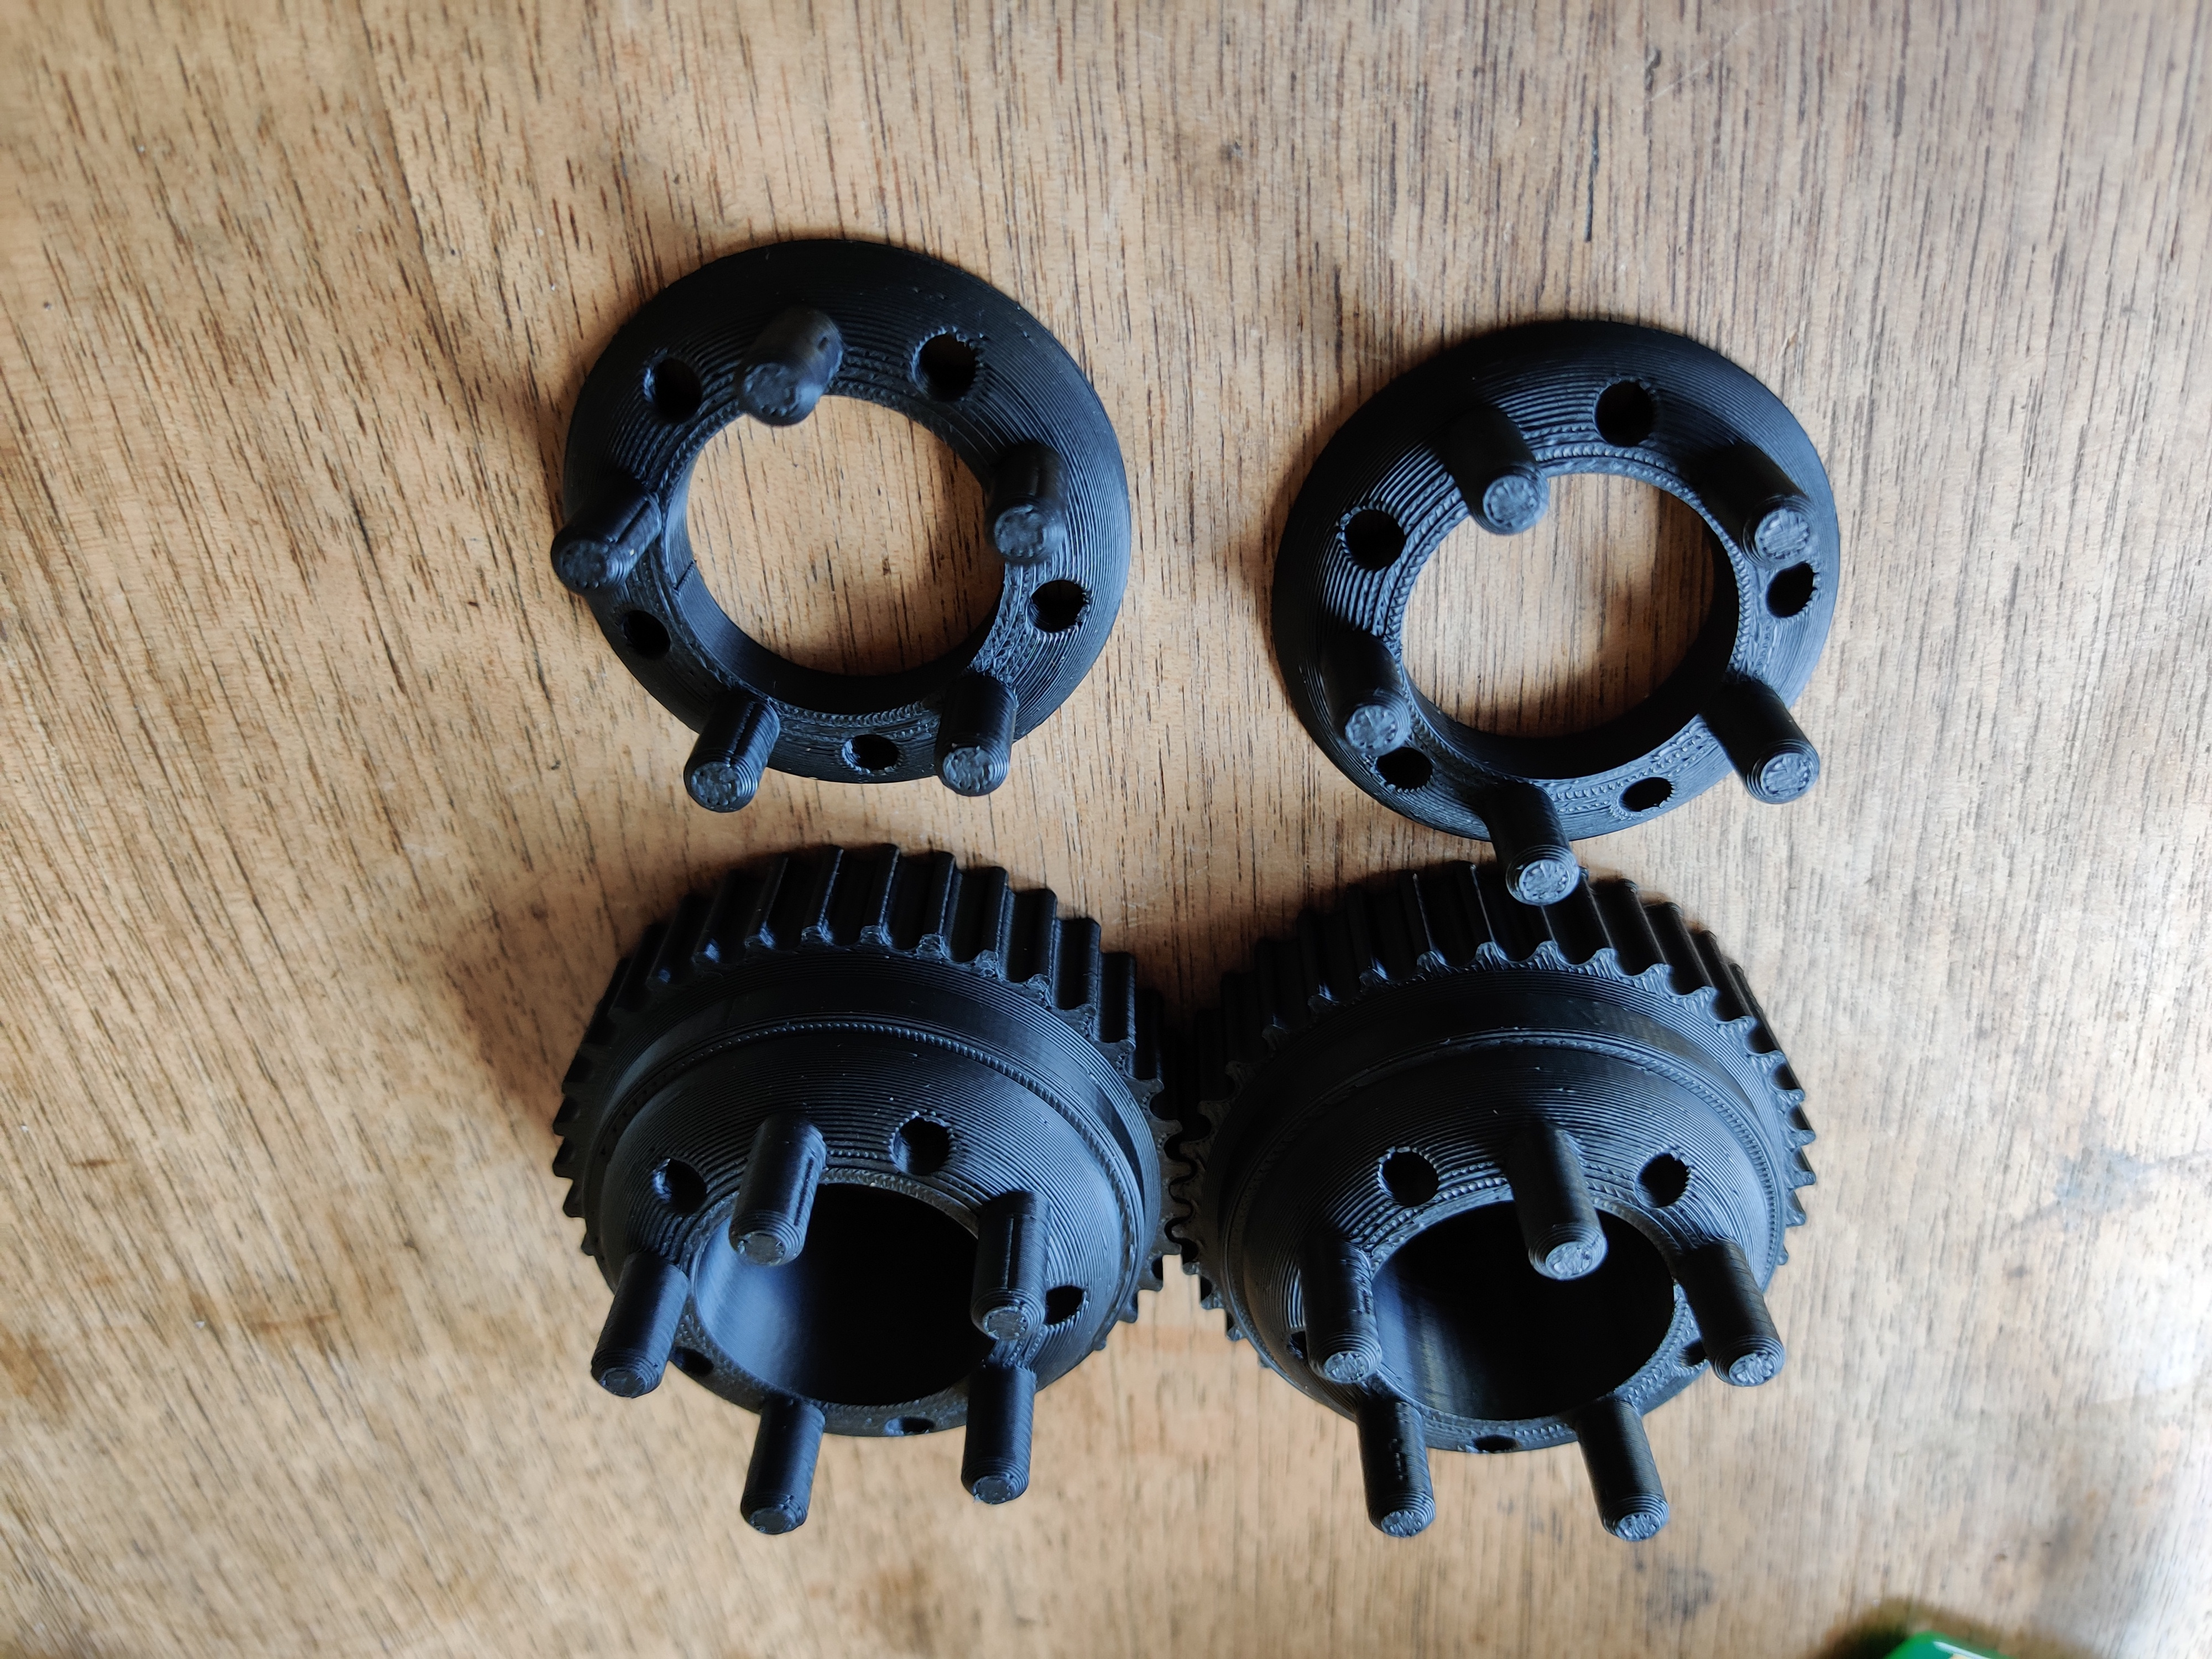
\includegraphics[angle=180, width=.49\textwidth]{Footage/Pictures/Wheel pulley v2.jpg}
			}
			\subcaptionbox{Zustand der Druckteile nach einigen Testfahrten.\label{subfig:printed pulleys after test driving}}[.49\textwidth][r]{
				\includegraphics[width=.49\textwidth]{Footage/Pictures/Wheel pulley v1.jpg}
			}
			\caption[Vergleich der gedruckten Zahn- und Konterscheiben vor und nach mehreren Testfahrten]{(a) Die finale und zum Zeitpunkt des Verfassens dieses Dokumentes noch verbaute Version. (b) Der Zustand des ersten funktionalen Prototypes nach etwa~\qty{100}{\kilo\metre} Testfahrt. Neben zu erwartender Verschmutzung sei insbesondere auf das Fehlen der Führungsstifte zu achten. Das Zahnprofil und die Komponenten als ganze weisen darüber hinaus jedoch keinerlei Anzeichen von Materialversagen auf.}
			\label{fig:comparison printed parts used unused}
		\end{figure}
		%
	\section{Kosten}\label{sec:cost}
		\begin{table}[h]
			\caption[Kostenaufstellung der Einzelteile]{Kostenaufstellung der Einzelteile. Da nicht alle Teile gekauft werden mussten sind wo zutreffend Schätzwerte angegeben.}%
			\label{tab:costs}
			\centering
			\begin{threeparttable}
				\begin{tabular}{lp{1cm}r}
					\toprule
					Teil											&& Kosten\\ \midrule
					Druckteile										&& \dEUR{2}\\
					Motorhalterungen\tnote{a}						&& \dEUR{170}\\
					\hspace{5mm}Nur Halbzeug						&& \dEUR{17,67}\\
					Motoren											&& \dEUR{177}\\
					Schrauben										&& \dEUR{3}\\
					Steckverbinder									&& \dEUR{2}\\
					Rollen\tnote{b}									&& \dEUR{34,75}\\
					Zahnriemen										&& \dEUR{29,4}\\
					Zahnriemenscheiben								&& \dEUR{19,6}\\
					&&\\
					\textbf{Gesamt}									&& \dEUR{455,42}\\
					\bottomrule
				\end{tabular}
				\begin{tablenotes}\footnotesize
					\item[a]	Fertigungsangebot inklusive Material.
					\item[b]	Preis für zwei Rollen.
				\end{tablenotes}
			\end{threeparttable}
		\end{table}
% LTeX: language=de-DE
\chapter{Zusammenfassung}
	Die geforderte Maximalgeschwindigkeit konnte zwar im Leerlauf weit übertroffen werden, im Rahmen von Feldtests unterlag sie jedoch leicht den geforderten \qty{25}{\kilo\metre\per\hour}.
	Da sie jedoch softwareseitig limitiert wurde und bei Erreichen der gemessenen Maximalgeschwindigkeit noch ausreichend Leistungsreserven zur Verfügung standen ist davon auszugehen, dass, mit geeignetem Personenschutz, höhere Geschwindigkeiten ohne weiteres erzielt werden können.
%-----------------------------------------------------------------
\newpage
\appendix
\chapter{Anhang}
	\begin{figure}[h]
		\centering
		\includesvg[width=\textwidth]{Assets/mosfets-Power MOSFETS}
		\caption[Schaltplan der Leistungsendstufe des ESC]{Schaltplan der Leistungsendstufe des ESC\cite{vesc.documentation.2015}.}
		\label{fig:power mosfets}
	\end{figure}
\printbibliography%
%=================================================================
\end{document}